\providecommand{\classoptions}{keys}
%% The next two lines are suggested at
%% to work around the following error:
%%
%%  ----------------------------
%%  /usr/local/texlive/2018/texmf-dist/tex/latex/chngcntr/chngcntr.sty:42: LaTeX Error: Command \counterwithout already defined.
%%                 Or name \end... illegal, see p.192 of the manual.
%%
%%  See the LaTeX manual or LaTeX Companion for explanation.
%%  Type  H <return>  for immediate help.
%%   ...
%%
%%   l.42 ...thout}{\@ifstar{\c@t@soutstar}{\c@t@sout}}
%%   ----------------------------
%%
%% The two lines:
\let\counterwithout\relax
\let\counterwithin\relax
%% Suggested fix above taken from
%% https://tex.stackexchange.com/questions/425600/latex-error-command-counterwithout-already-defined
%%

\documentclass[
  11pt,
  deliverables,
  longtasklabels,
  numericcites,
  noworkareas,
  svgnames,
  \classoptions
]{euproposal}       % for writing
%\documentclass[submit,noworkareas,deliverables]{euproposal}        % for submission
%\documentclass[submit,public,noworkareas,deliverables]{euproposal} % for public version

\usepackage[utf8]{inputenc}
\usepackage{hyperref}
\usepackage{enumitem}
\usepackage{booktabs}

% \usepackage{minitoc}
%\usepackage{varioref}

\usepackage{float}  % used to suppress floating of tables in Resources section.
\usetikzlibrary{calc,fit,positioning,shapes,arrows,snakes}
\graphicspath{{tasks/}}

\addbibresource{bibliography.bib}
% temporary fix due to http://tex.stackexchange.com/questions/311426/bibliography-error-use-of-blxbblverbaddi-doesnt-match-its-definition-ve
\makeatletter\def\blx@maxline{77}\makeatother

% \input{WApersons} % Some sections of the included files depend on this.
\usepackage{lscape} % for landscape
\usepackage{comments}
% %\usepackage[final]{comments}
\usepackage{fontspec}
\usepackage{verbatim}
\usepackage{listings}
\usepackage{supertabular,array}
\usepackage[breakable]{tcolorbox}
\makeatletter
\newcommand\arraybslash{\let\\\@arraycr}
\makeatother
% \setlength\tabcolsep{1mm}
% \renewcommand\arraystretch{1.3}
%% Related Projects
\newcommand{\scienceproject}{\mbox{\textsc{SCIEnce}}\xspace}
\newcommand{\OOMMF}{OOMMF\xspace}
\newcommand{\OOMMFNB}{OOMMF-NB\xspace}
\newcommand{\ODK}{OpenDreamKit\xspace}
\newcommand{\VRE}{VRE\xspace}
\newcommand{\VREs}{VRE\xspace}
\newcommand{\software}[1]{{#1}\xspace}
\newcommand{\GAP}{\software{GAP}}
\newcommand{\HPCGAP}{\software{HPC-GAP}}
\newcommand{\libGAP}{\software{libGAP}}
\newcommand{\Singular}{\software{Singular}}
\newcommand{\Sage}{\software{SageMath}}
\newcommand{\SageCombinat}{\software{Sage-Combinat}}
\newcommand{\MuPADCombinat}{\software{MuPAD-Combinat}}
\newcommand{\Docutils}{\software{Docutils}}
\newcommand{\Pygments}{\software{Pygments}}
\newcommand{\Sphinx}{\software{Sphinx}}
\newcommand{\SCSCP}{\software{SCSCP}}
\newcommand{\JavaScript}{\software{JavaScript}}
\newcommand{\Python}{\software{Python}}
\newcommand{\IPython}{\software{IPython}}
\newcommand{\Jupyter}{\software{Jupyter}}
\newcommand{\JupyterHub}{\software{JupyterHub}}
\newcommand{\BinderHub}{\software{BinderHub}}
\newcommand{\Cython}{\software{Cython}}
\newcommand{\Pythran}{\software{Pythran}}
\newcommand{\Numpy}{\software{Numpy}}
\newcommand{\Pari}{\software{PARI}}
\newcommand{\PariGP}{\software{PARI/GP}}
\newcommand{\libpari}{\software{libpari}}
\newcommand{\GP}{\software{GP}}
\newcommand{\GPtoC}{\software{GP2C}}
\newcommand{\Linbox}{\software{LinBox}}
\newcommand{\LMFDB}{\software{LMFDB}}
\newcommand{\OpenEdX}{\software{OpenEdX}}
\newcommand{\Linux}{\software{Linux}}
\newcommand{\LATEX}{\software{\LaTeX}}
\newcommand{\SMC}{\software{SageMathCloud}}
\newcommand{\cocalc}{\software{CoCalc}}
\newcommand{\Simulagora}{\software{Simulagora}}
\newcommand{\KANT}{\software{KANT}}
\newcommand{\Magma}{\software{Magma}}
\newcommand{\Mathematica}{\software{Mathematica}}
\newcommand{\Maple}{\software{Maple}}
\newcommand{\Matlab}{\software{Matlab}}
\newcommand{\MuPAD}{\software{MuPAD}}
\newcommand{\MPIR}{\software{MPIR}}
\newcommand{\Arxiv}{\software{arXiv}}
\newcommand{\Givaro}{\software{Givaro}}
\newcommand{\fflas}{\software{fflas}}
\newcommand{\MathHub}{\software{MathHub}}
\newcommand{\FindStat}{\software{FindStat}}
\newcommand{\GitHub}{\software{GitHub}}
\newcommand{\GitLab}{\software{GitLab}}
\newcommand{\Trac}{\software{Trac}}
\newcommand{\git}{\software{git}}
\newcommand\DKS{\ensuremath{\mathcal{DKS}}\xspace}
\newcommand{\FLINT}{\software{FLINT}}
\newcommand{\nbval}{\software{nbval}}
\newcommand{\nbdime}{\software{nbdime}}
\newcommand{\nbdiff}{\software{nbdiff}}
\newcommand{\nbmerge}{\software{nbmerge}}
\newcommand{\conda}{\software{conda}}
\newcommand{\clang}{\software{clang}}
\newcommand{\gcc}{\software{gcc}}
\newcommand{\cling}{\software{cling}}
\newcommand{\Julia}{\software{Julia}}
\newcommand{\Fortran}{\software{Fortran}}

\XeTeXtracingfonts=1\relax

% this is latex's Times New Roman,
% extending Nimbus Roman No9 L
\setmainfont[
    Extension=.otf,
    UprightFont=*-regular,
    BoldFont=*-bold,
    ItalicFont=*-italic,
    BoldItalicFont=*-bolditalic,
]{texgyretermes}

\usepackage{framed}
\usepackage{multicol}
\usepackage{lipsum}

\newcommand{\allparticipants}{{SRL,MP,QS,UIO,IFR}}

\newcommand{\softwarename}[1]{\texttt{#1}}
\newcommand{\repotodocker}{\softwarename{repo2docker}}
\newcommand{\binderhub}{\softwarename{BinderHub}}
% \newcommand{\mybinder}{\softwarename{mybinder.org}} % mybinder.org in monospaced font
\newcommand{\mybinder}{mybinder.org}   % mybinder.org in normal proportional
% font
% \newcommand{\myemph}[1]{\emph{#1}}%    to try bf or emph in ambition section
\newcommand{\myemph}[1]{\textbf{#1}}%    to try bf or emph in ambition section

\newcommand{\noemph}[1]{#1}%    to switch off emphasis but keep the option to
                           %    de-activate it again later

%\newcommand*{\fullref}[1]{\ref{#1} \nameref*{#1}} % One

\newcommand*{\fullref}[1]{\hyperref[{#1}]{\ref{#1} \nameref*{#1}}}
% single clickable link of the style: 1.1 Concept
% source: https://tex.stackexchange.com/questions/121865/nameref-how-to-display-section-name-and-its-number



% longtaskref: T1.2: Title of task
\newcommand\longtaskref[2]{\csname task@#1@#2@label\endcsname: ``\csname task@#1@#2@title\endcsname''}



\begin{document}

% satisfy fancyhdr with 11pt
\setlength{\headheight}{13.6pt}

\begin{draft}

\section*{Guidelines for proposal co-authors}

\begin{verbatim}
- Consistency.
  - [ ] Section or section or Sect or Sec? Use 'Section'
  - [ ] Figure or figure or Fig or Fig.? Use 'Figure'
  - [ ] Binder or binder - Binder? Use 'Binder'
  - [ ] MyBinder or Mybinder or mybinder? Use `mybinder.org` for the public
        instance of the service -> \mybinder

- we have a command \repotodocker to insert 'repo2docker' in \softwarename{}
  font.
- we have a command \binderhub to insert 'BinderHub'.
- we have a command \mybinder to insert 'mybinder.org'.
- Best use {} after the commands to enforce a space, i.e. ``\repotodocker{} is the focus''


- to discuss
  - ONHOLD [ ] names of work packages. Section 3.1.1
    - [X] Management
    - [ ] Core  -> enhancement? Robustness?
    - [ ] Impact -> new features? Increase impact?
    - [ ] Applications -> Use cases?
    - [ ] Education -> Dissemination? Education and Outreach?

    Hm, the long names see okay. Need to investigate where I got the short names
    from.



- This nice section could be included in our approach (1.2.10):

  Facilitating Open and Reproducible Science by automating existing practices &
  A key to our philosophy and success thus far has been automating
  what scientists already are (or should be) doing.
  The approaches and environment specifications used in Binder are
  not specific to Binder, and are already widely adopted.
  We only seek to automate this process,
  and implement and document as many standards as we can find in use by the community.
  By implementing what is already in use,
  we minimise "lock-in" and meet users,
  lowering the barrier to adoption relative to "bespoke" tools,
  which require a large change in tooling, and significant disruption to researchers'
  work.

- [x ] Check size limit for pdf to upload (was it 10MB? Can be seen at upload
      menu in portal). => It is 10MB
  - [ ] check size of final.pdf => it is 4.1 MB now.18.04.17:23 
  - [ ] if size is a problem, we can downsample the 'spectrogram.png' image.

- [ ] mention reference (discretisedfield?) for interactive documentation
      in text.

- [ ] fix XXX-XX-XXX in telefon fax 
       => I do not think we need to put telfon fax here as it is in PartA. 
- [ ] in Part A : ' Has this proposal (or a very similar one) been submitted in the past 2 years in response to a call for proposals under any EU programme, including the current call?'
it is ticked as yes for this, but proposal reference or contract number is not indicated.  Who have the info? 


- [ ] add phone, website of Min at partA?

- [ ] update Keywords on title page of part B
- [ ] copy the keywords & abstruct to PartA (EU portal) 
\end{verbatim}

\section*{Todo items}
- [ ] describe our relation to the Binder team

\end{draft}
\draftpage

\begin{proposal}[
  % participants
  PI=mrk,
  mrkname=Benjamin Ragan-Kelley,
  mrkaffiliation=Simula Research Laboratory,
  mrkdept=Numerical Analysis and Scientific Computing,
  mrktitle=Dr.,
  % site descriptions
  site=SRL, % Simula
  SRLacronym=Simula,
  SRLshortname=Simula Research Laboratory,
  SRLcountryshort=NO,
  SRLcountry=Norway,
  site=MP, % Max Planck
  MPacronym=MPG,
  MPshortname=Max Planck Gesellschaft,
  MPcountryshort=DE,
  MPcountry=Germany,
  site=QS, % QuantStack
  QSacronym=QuantStack,
  QSshortname=QuantStack,
  QScountryshort=FR,
  QScountry=France,
  site=IFR, % Ifremer
  IFRacronym=Ifremer,
  IFRshortname=Ifremer,
  IFRcountryshort=FR,
  IFRcountry=France,
  site=UIO, % U Oslo
  UIOacronym=UiO,
  UIOshortname=University of Oslo,
  UIOcountryshort=NO,
  UIOcountry=Norway,
  % site=XXX, % template example
  % alternative: (can be combined)
  coordinator=Simula Research Laboratory,
  Cemail=benjaminrk@simula.no,
  Ctelfax=(47) XXX-XX-XXX,
  %coordinatorsite=SRL,
  acronym={SOURCE},
  acrolong={SOURCE},
  proposalnumber={SEP-210850361},
  title={Supporting Open, Useful, and Reproducible Computational Environments},
  callname=Increasing the reproducibility of scientific results,
  callid=WIDERA-2022-ERA-01-41,
  % TODO: consistency with provided template
  % CALL: H2020-EINFRA-2015-1
  % TOPIC: e-Infrastructures for Virtual Research Environments (VRE)
  % Instrument: e-Infrastructures
  keywords={
  Open Science,
  reproducibility,
  reusability,
  education,
  accessibility,
  Jupyter,
  Binder,
  notebooks,
  cloud,
  EOSC,
  HPC,
  FAIR data,
  geosciences,
  health sciences,
  photon science
  },
  % computational mathematics,
  % GAP, Linbox, PARI, Sage, Singular, IPython, Jupyter, SageMathCloud, LMFDB, MathHub
  % Virtual research environments, MPIR, /GP
  % open source, free software, number theory, abstract algebra, notebooks
  instrument= Call: HORIZON-WIDERA-2022-ERA-01-41, %Call: H2020-EINFRA-2015-1, 3 Topic 9-2015
  challengeid = TODO,
  %challenge = {N/A},
  %objectiveid={N/A},
  %objective = TODO,
  %outcomeid = N/A,
  %outcomet = N/A,
  months=36,
  compactht]
\newcommand{\TheProject}{\pn}% \pn is defined automatically
% \input{grantagreement-history}

\ifsubmit
\else
% only abstract in draft
\draftpage
\input{abstract}

% detailed toc in draft
\setcounter{tocdepth}{4}
\fi

\tableofcontents

% ---------------------------------------------------------------------------
%  Section 1: Excellence
% ---------------------------------------------------------------------------

\section{Excellence}
\eucommentary{4 pages}
\eucommentary{\emph{
\begin{itemize}
\item Briefly describe the objectives of your proposed work. Why are they pertinent to the work programme topic? Are they measurable and verifiable? Are they realistically achievable?
\item	Describe how your project goes beyond the state-of-the-art, and the extent the proposed work is ambitious. Indicate any exceptional ground-breaking R-and-I, novel concepts and approaches, new products, services or business and organisational models. Where relevant, illustrate the advance by referring to products and services already available on the market. Refer to any patent or publication search carried out.
\item	Describe where the proposed work is positioned in terms of R-and-I maturity (i.e. where it is situated in the spectrum from idea to application, or from lab to market). Where applicable, provide an indication of the Technology Readiness Level, if possible distinguishing the start and by the end of the project.
\end{itemize}
Please bear in mind that advances beyond the state of the art must be interpreted in the light of the positioning of the project. Expectations will not be the same for RIAs at lower TRL, compared with Innovation Actions at high TRLs.
}
}
\medskip

\subsection{Objectives and ambition}

\label{sect:objectives}

As the values of \textbf{open science} and \textbf{reproducible science} are adopted by
governments, funding agencies, research institutes, and society,
there are practical challenges to implementing such practices on a global scale.

Two of the key societal goals of open science are facilitation of
\begin{compactitem}
\item \textbf{verification} of results, improving the reliability and trustworthiness of scientific output, and
\item \textbf{reuse} of research products, enabling commercial exploitation and/or derivative research.
\end{compactitem}

\noindent If results are merely \emph{available}, however,
much of the value of Open Science remains unrealised.
\myemph{Practical reproducibility} is required for efficient, widespread fulfilment of Open Science goals.
But what does it mean to be reproducible?
Without the \myemph{practical} ability to verify results, results are not
any more likely to be verified.
Without the \myemph{practical} ability to reuse work, results are not
any more likely to be exploited in new research or commercial work.

In \TheProject, we focus on ``practical reproducibility'',
specifically focusing on computational results, such as computer simulation, data
processing, data analysis, and creation of figures and tables in publications.
We differentiate ``technical reproducibility'',
where enough information is \emph{technically present} to reproduce the work given sufficient effort,
from ``practical reproducibility''
where effort to reproduce the work is not a burden~\cite{binder}.

\subsubsection{Ambition}

Computational reproducibility is a major challenge facing all scientific domains,
from social sciences to life sciences, physical sciences, engineering, and digital humanities.
Almost every area of academia must spend some time computing,
ranging from large-scale computer simulations to basic data analysis to produce a figure in a publication.

All of these face a common reproducibility challenge: \textbf{the computational environment},
or the collection of software used to produce the output.
To reproduce the work, a \textbf{sufficiently similar} computational environment must be produced to re-execute the code.
This may be a specific version of an application, or a large collection of software dependencies,
as is common in data science fields.

In order to meet the goals or policies of open and reproducible science,
\myemph{researchers need tools} to address the challenge. Ideally, those tools should
\begin{compactitem}
\item be freely available and open source (to maximise access and longevity); and
\item meet researchers where they are, as much as possible (to maximise practical adoption).
\end{compactitem}

\TheProject's main goal is to \myemph{improve the global reproducibility of
  scientific results} with a focus on those aspects of the research process that
are supported by computation and software, such as computer simulation, data
processing, data analysis and creation of figures and tables in publications.

We plan to achieve this goal through
\begin{compactitem}
\item educating researchers about good reproducible practices, and
\item making it easier to perform computational research in a reproducible way
  through improving and developing relevant software tools.
\end{compactitem}

Rather than re-inventing the wheel, we will build upon \textbf{existing tools and standards}.

Increasingly, open science and reproducibility are declared as values or requirements
at research institutions, governments, and funding agencies.
In order to meet these goals or requirements,
researchers need \myemph{tools} that help them accomplish the tasks required for reproducible work.

It is in this context that we set our objectives to \textbf{develop, experiment with, and mainstream Binder tools as concrete solutions and best-practices to increase the reproducibility of research}:

\begin{table}[H]
  \begin{tabular}{>{\raggedright}m{.2\textwidth}|m{.36\textwidth}|m{.36\textwidth}}
    \toprule

    \myemph{Objective} & \myemph{Description} & \myemph{Relation to work programme}\\\midrule

    \label{obj:reproducibility} Objective 1:\\\medskip \myemph{Evaluate and facilitate better computational
    reproducibility and FAIR data}
    &
    Tools for reproducibility must be evaluated by how successfully they produce the correct environment.
    We will provide evaluation tools for reproducibility,
    and use these tools to guide improvements to the Binder tools,
    solving known issues where we can improve the \myemph{reproducibility of computational environments}
    used for science, and facilitate \myemph{FAIR data practices}.
    &
    The core of this effort is to \textbf{develop, validate, pilot, and deploy practices and practical tools for funders, publishers, and scientists}.
    The robustness of these tools is key to their utility and value,
    and thereby adoption in research communities.
    \\\midrule

    \label{obj:broaden} Objective 2:\\\medskip
    \myemph{Enable reproducibility using common tools in a wider variety of environments}
    &
    We develop \textbf{generic tools for reproducible software environments},
    but have identified several areas where the Binder tools do not yet meet user needs,
    such as traditional \textbf{HPC environments}, or users with \textbf{large datasets}.
    We shall address those gaps so that tools and strategies can be shared by a wider variety of communities,
    aligning effort and reducing necessary duplication.
    &
    In order to \textbf{promote uptake, greater collaboration, and increased alignment of the activities of stakeholders},
    it is most efficient when knowledge and tools can be shared.
    When tools do not work for significant fractions of the research community,
    they must develop their own, often similar tools,
    as has often been the case e.g. for the HPC community.

    \\\midrule

    \label{obj:demonstrators} Objective 3:\\\medskip
    \myemph{Demonstrate reproducibility in specific scientific applications}
    &
    We will demonstrate the utility of the Binder tools for achieving reproducible research
    in a variety of scientific domains,
    which serves both to \textbf{inform and motivate} improvements to the system,
    and as \textbf{illustration and reference} for others to follow.
    &
    By collaborating across domains, we \textbf{promote uptake, greater collaboration, and increased alignment of the activities of stakeholders}.
    Further, by publishing working examples,
    we contribute to an \textbf{open knowledge base of results, methodologies and interventions on the drivers and consequences of reproducibility} in these specific domains,
    to be used as reference or followed by others in the same domain
    and other domains with similar challenges.

    \\\midrule

    \label{obj:education} Objective 4:\\\medskip
    \myemph{Educate researchers about reproducible practices}
    &
    Develop \textbf{best practice guidelines} for reproducible science, and disseminate this by
    \textbf{educating the research communities} about reproducible practices and available
    tools for reproducible publications and policies. \textbf{Reach out} to scientists, and
    the wider research communities and reproducibility stakeholders to encourage
    engagement with this project.
    &
    By collecting expertise and guidelines, we contribute an \textbf{open knowledge base of results, methodologies and interventions}
    for computational reproducibility.
    \\\bottomrule

  \end{tabular}
  \label{tab:objectives-tasks}
  \caption{
    Our objectives and their relationship to the work programme}
\end{table}

\subsubsection{Binder tools for reproducible research}
\label{sec:reproducibility-example}

Binder\footnote{\url{https://jupyter.org/binder}} is a project providing open source tools to solve this computational environment reproducibility challenge.
It has already proven useful for at least tens of thousands of researchers, educators, developers, and students,
and we believe it has the potential to \textbf{facilitate practical reproducibility for millions} more,
including in institutions, funding agencies, and policy makers.
We aim to realise that potential by extending Binder open source tools.

\begin{figure}[htb]\centering
  \includegraphics[width=0.9\textwidth]{use-cases-binder-logbook-solution.png}
  \caption{A typical use case for Binder-based reproducibility using Jupyter notebooks in research.
            Image by Juliette Belin for the OpenDreamKit project, used under
            CC-BY-SA.}\label{fig:use-cases-binder}
\end{figure}

We start with an example making use of existing \textbf{Binder
tools for computational reproducibility}. Starting from this base-line, we can
explain what progress and additional impact we will enable through this project.

Figure~\ref{fig:use-cases-binder} depicts how a scientist can use a Jupyter
notebook and the Binder software to make her research results easily
reproducible and reusable. Jupyter notebooks are popular with millions of researchers and allow the creation of notebook
documents, containing a mixture of text and interactively executable code, along with rich output from
running that code. In short:
\begin{compactitem}
\item Scientist Jane has created a \myemph{notebook that carries out computations} or
  data processing and creates a figure based on those results. For the purpose
  of the introduction of this workflow, we assume that
  Figure~\ref{fig:reproducibility-example-covid} shows this figure.

\item She has made the notebook and raw data available in a \myemph{public repository}
  (for our example at\newline
  \mbox{\url{https://github.com/fangohr/reproducibility-repository-example}}).

\item As she has described \textbf{what software is needed} to execute her notebook (more
  details below), it is possible for all interested scientists (and anybody
  else, including the reviewers of this proposal) to \myemph{reproduce} her
  figure.

  To reproduce the figure, one needs to visit an online
  URL\footnote{\url{https://mybinder.org/v2/gh/fangohr/reproducibility-repository-example/HEAD?labpath=figure1.ipynb}}
  (which contains a combination of the public repository and online Binder service adress)
  in a browser, and then wait a minute or so for a dedicated computational
  environment to be created and started. Then select ``Run'' -> ``Run all cells''
  from the menu of the interactive Jupyter notebook that will appear in the
  browser.


  At that point, the \textbf{computational steps} that Jane has carried out
  \textbf{to create her
  results are repeated}, and the results are \myemph{reproduced}.

  (We provide a more detailed description of the components and steps in this
  process in the Section~\ref{sec:opensource}.)

\item Because all the computational steps are captured in the Jupyter notebook,
  they can be inspected and interrogated if desired. In particular, the steps
  can be modified and re-executed: this allows very efficient \myemph{re-use} of
  the results by other researchers.
\end{compactitem}


The reproducibility workflow shown in Figure~\ref{fig:use-cases-binder} is
working today, and we provide estimates on the number of current users in
section \ref{sec:mybinder}. The work proposed for this project will build on
this existing technology and (i)~make it \myemph{more robust and easier to use}
(\WPref{reproducibility}), and (ii)~extend the functionality (\WPref{impact}) so
that the existing tools can be \textbf{used in many more use cases}
(\WPref{applications}).

We note in particular that the Binder-enabled workflow for reproducibility has
originally been developed to reproduce results that are created within Jupyter
notebook (as shown in Figure~\ref{fig:use-cases-binder}).
However, \textbf{the approach taken is generic, and not specific to notebooks}: it is
based on \repotodocker{} (Section~\ref{sec:repo2docker}), a tool to \textbf{build, run, and
publish} Docker images from source code repositories.
As part of this project, we will demonstrate that reproducible
computational environments can be created using the same approach
in studies that do not make use of Jupyter notebooks.

\begin{figure}
  \centering
  \includegraphics[width=1.0\textwidth]{images/figure1.pdf}
  \caption{Figure (\softwarename{figure1.pdf}) which can be reproduced in our explanatory repository example
    \cite{ReproducibilityRepositoryExample2022}. \label{fig:reproducibility-example-covid}}
\end{figure}


\subsubsection{State of the art}

To make computational research \textbf{reproducible}, we generally need to make available
(i)~required \textbf{data}, (ii)~the required \textbf{software}, (iii)~the \textbf{protocol} that explains
how to process the data to obtain the result that is to be reproduced. Using
services such as Zenodo, it is possible to deposit such archives with a DOI and
make reference to them in publications.

In order to reproduce the results, it should be possible for anybody to take such an archive of a research
output, and to carry out the two necessary steps:
\begin{compactitem}
\item Step 1 to install the required software, and
\item Step 2 to follow the protocol to reproduce the results from the archived data.
\end{compactitem}

It is of particular value if Steps 1 \emph{and} 2 can be \emph{carried out
  automatically} by executing a program included in the
archive. First, if the automatic execution is possible, we know that there is a
complete description of the protocol included in the archive, and that no
mistake is made in trying to follow the protocol. Second, the automatic
execution saves time.

There are two common approaches to achieve this reproducibility: (a) to use a
\textbf{workflow} tool or environment that caters to a given use case (for
example~\cite{Afgan2018,Mlder2021,reana2019})
and encapsulates the full process for strong reproducibility guarantees,
or (b) to use \textbf{standard} (software engineering) \textbf{computing tools} and conventions
(git, make, python, perl, bash, \ldots)
to specify the compute environment and reproduce steps piecemeal.

The workflow tool approach (a) is robust, but requires ``all-in'' adoption by authors and reproducers alike,
and is \textbf{difficult in practice}. It can also have associated ``vendor lock-in'' effects
--- once a tool is adopted for one piece, it must be used for all associated work.
A consequence of this more tailored approach is \textbf{reduced re-use and duplication of effort}.
As a workflow tool may not meet the needs of a community,
that community must then build its own tool, or be left \textbf{without appropriate tools}
if they lack the resources or expertise to build their own.
Workflow tools also often \emph{dictate} a significant amount of how researchers perform their work,
which can inhibit adoption of the workflow tool by researchers
when it does not suit their existing patterns.

The \textbf{standard computing tools} approach (b) is generic, but \textbf{not accessible} to all researchers
as it requires substantial training or experience to be effective,
and it is prone to errors or incompleteness when executed,
leading to the ``Works for Me'' problem:
the author may have no trouble reproducing their own work,
but they have not effectively communicated the requirements such that others can do the same.
The \textbf{gap between researchers' expertise and practical need} when it comes to these tools has led to the creation
of whole industries of remedial skills training.
The loose coupling of tools and modular choices make it \textbf{more flexible} (covering more use cases),
but \textbf{more difficult} to follow robustly.
Identifying which tools to use and following appropriate installation is a challenge
for both authors, who must communicate requirements clearly without knowing the reader's context,
and readers, who must find, understand, and follow potentially complex directions, even assuming they were
complete and correct.

\medskip Researchers who use the Jupyter notebook to orchestrate their
computational research can achieve this automatic
reproducibility with little additional effort~\cite{Beg2021}: they use the notebook document as
the protocol of their analysis (Step 2), which can be executed automatically.
They can make use of the \textbf{Binder tools} (Section~\ref{sec:opensource}) and/or the
associated  mybinder.org\footnote{\url{https://mybinder.org}} service (free and public) that has
been designed by the Jupyter team to \textbf{automatically create the appropriate
software environment} (Step 1) in which the notebook can be executed.
But different workflows and tools are not as well served, yet.

BinderHub instances such as mybinder.org are extremely convenient,
but being hosted services they do not offer the autonomy
of private execution on one's own computational resources,
be they a local machine or cloud or on-premises clusters.

\subsubsection{Beyond the state of the art}

In this project, we will focus on the \myemph{reproduction of the
software environment} (Step 1) which is a prerequisite for any attempt to
reproduce the actual research outputs. In particular, we want to make the
creation of this computational environment \myemph{automatic}, \myemph{generic} and \myemph{robust},
especially for long-term preservation.

We will go beyond the current state of the art by bringing the following selected improvements:
\begin{compactitem}
\item Currently, producing valid computational environments from published scientific publications and/or existing
      online repositories is difficult and usually requires manual handling of the process which is cumbersome and
      time consuming. \textbf{Improving the robustness of Binder tools} and in particular \repotodocker{}'s ability to
      produce computational environments long after the publication and/or
      release ---
      through testing and development, as well as taking additional context information into account,
      such as repository publication date --- will \textbf{enable seamless
        reproduction of computational environments};
\item The existing \textbf{Binder tools} are already widely used in the Jupyter user community,
      but the focus has been on the reproducibility of Jupyter notebooks that may not fit everyone’s needs.
      Highlighting and extending \textbf{Binder tools}' \textbf{capabilities beyond notebooks}
      will undoubtedly \textbf{attract new communities} of users and can facilitate
      \textbf{transfer of knowledge} between academia and industry;
\item The current Binder tools rely on Kubernetes and deploying a Binder service requires technical skills that are
      beyond many institutional or companies IT support staff. As a result, most researchers rely on existing
      deployments that are overloaded and cannot cope with the huge demand, and they may disregard Binder
      as a viable solution for creating reproducible computational environments. \textbf{Being able to use \repotodocker{}
      anywhere} e.g. from the user’s personal laptop (Binder@home, \taskref{applications}{binder-at-home}) to the
      most powerful supercomputers (Binder@HPC, \taskref{applications}{binder-at-hpc})
      by removing technical restrictions such as the dependence on Kubernetes,
      and supporting a wider variety of community practices for reproducible environments
      will open new ways of using Binder tools that are more in line with the current needs of end-users;
\item Another important bottleneck is the need to \textbf{access and to reuse very large and complex datasets} (sometimes
      with restricted access permissions) that are published and deposited on (domain-) specific long-term archives.
      Specific use cases (to read and process such datasets) are provided by end-users (either as part of the dataset
      itself or separately) but the usage of the Binder software and/or existing public Binder deployments for
      this use case is not yet well supported (such amount of data cannot be easily and efficiently moved to
      public Binder instances).
      \emph{Ad hoc} or domain-specific solutions (for instance the usage of cloud optimized
      data formats and associated catalogs such as intake\footnote{\url{https://intake.readthedocs.io/en/latest/index.html}}
      or STAC\footnote{\url{https://stacspec.org}} by the Pangeo\footnote{\url{https://pangeo.io}} Geoscience community)
      have been explored by diverse communities but are technically difficult and not generic enough to be
      adopted by everyone. The Binder software will be extended to \textbf{facilitate data publishing} (see \taskref{applications}{data-publishing}) with
      the plugin of external long-term archive resources and enable the \textbf{publication and reuse of large and complex datasets}.
\end{compactitem}


\subsubsection{Motivation --- why?}\label{sec:motivation-why}

We focus on the \textbf{computational reproducibility} because it is a real
obstacle for \textbf{practical reproducibility}.

First, it affects the majority of all researchers: there are estimates that \textbf{over
92\% of all researchers} work with research software and over 50\% develop
their own~\cite{Hettrick2014}. Where experiments drive the research, this is
often data processing, analysis, and plotting. Each of those computational
research cases needs a \textbf{software environment} in which the actual processing can
be carried out. The software environment may consist of somewhat standard
packages (for example use of a Python, R, or Julia plotting library), or it may
include tailored programs that have been developed specifically for a study.

Second, software packaging and management is a technically challenging topic,
and \textbf{we cannot expect 92\% of all researchers to master it} -- so we believe there
is a clear need to support them with appropriate tooling.

The complexity arises in parts from the increasing age of archived studies, and
also in the often unusual combinations of research software and libraries that
need to be combined for a particular study. Other difficulties include that a
reproduction typically needs to be done on a different computer, perhaps even on
a different operating system. If, say, a plotting library is used, then it may
change its interface or behaviour over time, so it is important to install
exactly the right version of the plotting library, before a reproduction of
results is attempted using it.

Third, being able to recreate the appropriate \textbf{software environment is} a
\textbf{prerequisite} before any actual reproduction of results can be attempted: it
would be inefficient to educate researchers what data and programs to archive,
if in the future nobody (or only very few highly trained people) will be able to
execute those scripts.

Fourth, there are low-hanging fruits: the work proposed here will
make it possible to create computational environments \textbf{automatically for
existing data archives}: the Binder philosophy is to support existing standards for software
specification, and to automatically build a software environment based on those standards.
Where researchers have used the existing software specification already, Binder tools
will work immediately on their archived files. This means that (i)~a researcher
putting together a well-organised archive does not need to know about Binder tools,
yet the researcher who wants to reproduce the results later can use Binder tools to
automate the recreation of the software environment. This also means that
(ii)~improvements we propose in this work, will make some existing archives (that
have been created in the past) more easily reproducible.

Finally, by popularising the standard practices, a \textbf{benefit} is achieved fully
\textbf{beyond the community we reach directly}.

%(It is part of our training programme to educate about the importance and methods
%for software specification.)

% \input{excellence.tex}
% \subsection{Objectives and ambition}
% \input{ambition.tex}
% \draftpage
% \input{objectives}
% \draftpage
% \input{relation_to_the_work_programme.tex}

% ---------------------------------------------------------------------------
%  Section 1.2: Methodology
% ---------------------------------------------------------------------------
\draftpage
\TOWRITE{Min/Hans}{Mention KPIs somewhere?}

\subsection{Methodology}\label{sec:concept_methodology}
\eucommentary{5-8 pages}

% \subsubsection{Concept}%\label{sec:concept}
%
% Open science is the principle that science, in order to be most
% {impactful} and {socially responsible}, should be done
% {publicly}, with as much of the scientific process and products
% accessible, reviewable, reproducible and reusable by as many members of
% the global community as possible.
%
% There are exciting opportunities for open science for almost all academic fields
% in the modern age of computational science. As more and more research takes the
% form of code and/or data, the opportunity to share, reproduce, and reuse
% scientific work is greater than ever, even enabling new forms of
% {interdisciplinary collaboration}, and interoperable and reusable results and
% tools.
%
%  Simultaneously, there are obstacles -- both technical and social -- to
% making open science and reproducible science a practical reality. The challenges
% include: If a researcher has code and/or data to publish, how is that best
% done? How do researchers learn {best practices for reproducible science} in
% their field? How do previously disconnected fields benefit from each other's
% work as the same computational challenges are faced again and again by different
% communities? How can scientists be encouraged to make their work reproducible?
%
% These are the questions that guide the \TheProject{} project.

\paragraph*{Supporting Open, Useful, and Reproducible Computational
  Environments (SOURCE)}\label{sec:SOURCE}

  \mbox{}\\

  The ideas behind our project title:
\begin{itemize}
\item The work done in \TheProject will be \textbf{Supporting} scientists in their
  endeavours to make their work more reproducible and reusable.
\item We believe in the value of \textbf{Open} science and \textbf{Open} source software.
  The best reproducibility and reusability of scientific results is given through
  complete transparency of the steps taken in the derivation of a result. For
  the computational aspects this means making all simulation and/or
  post-processing and analysis steps open source. While this may not always be
  possible, we advocate such openness as the best practice for reproducible science.

  All work done, including software, training, and documentation materials, will
  be open source and available through an open access license. (We note that the
  collective development of the grant proposal you are reading is also done as
  open source, and can be inspected at {\footnotesize \url{http://github.com/minrk/horizon-widera-2022}}.)

\item Measures towards better reproducibility have to be \textbf{Useful} and
  practical: if a proposed approach or tool burdens the scientist with
  additional work, or requires significant additional skills, it becomes less
  likely to be widely accepted.

  The philosophy we support here is that the proposed (Binder) tools for
  reproducibility are based on existing standards which are already
  adopted by many and considered best practices.

\item Within the wide field of reproducibility in science, we focus this
  project on the improvement of the automatic generation of \textbf{Reproducible
    Computational Environments}.
  % It is an essential step for reproducible
  % science to be able to setup the correct
  % software environment, before any attempt can be undertaken to reproduce (and
  % thus repeat) the calculation of a result obtained before.
\end{itemize}

\subsubsection{Outline of concept and approach}

In the following sections, we explain our concept and the technology on which this
proposed project builds in more detail.
\begin{itemize}
\item Sections~\fullref{sec:reproducibility} and
  \fullref{sec:reproducibility-challenges} contextualise the proposed work
  within the wide field of reproducibility.
% \item We illustrate the reproducibility discussion in
%   \fullref{sec:reproducibility-example} and highlight the current shortcomings
%   in \nameref{sec:reproducibility-challenges}.
\item Section~\fullref{sec:methodology} presents our approach to improving reproducibility.
\item We provide details on some of our science use cases in
  \fullref{sec:science-applications}. These studies will provide feedback to the development of the
  Binder tools, validate the tools, and serve to showcase the outcomes of
  \TheProject.
\item We provide some technical background and context for our implementation in \fullref{sec:opensource}.
\item Section~\fullref{sec:community-engagement-panel} presents our strategy to
  engage with all stakeholders in reproducibility in science. We use the forum to
  share requirements, constraints, and experiences from different communities,
  and to learn from each other. This will help us to
  create training materials that target different audiences and
  contribute to a relevant presentation of best practices.

\end{itemize}

\medskip

\subsubsection{Reproducibility}\label{sec:concept}\label{sec:reproducibility}

Before describing the focus of the work that we propose here, we want to embed
this into the much wider context of \textbf{reproducibility challenges}.

We will exclude the challenges of reproducing \emph{experimental} data. Our
study starts at the point where such experimental data is available in digital
form.

We will focus on the challenge of \textbf{computational reproducibility}: can we carry out
the same data analysis or creation of figures and tables as they are presented in
a paper, at a later stage, and get to the same results?

Such tables and figures in a publication may be computed from the analysis of
some type of raw data which could originate from an experiment, another publication,
a data base, post-processing of another dataset or from executing computer
simulations.

% Where additional software, such as analysis scripts, input files
% and software for the simulation are needed,

\subsubsection{Challenges of reproducibility}\label{sec:reproducibility-challenges}

We can classify the reproducibility challenges listed above into different categories:

\begin{description}
\item[1. Workflow:] Are the processing commands (and their order)
\textbf{correctly recorded}? Do we know which part of the dataset the analysis is meant to be applied to? Do we know the protocol, \emph{i.e.} are the different processing steps for that data recorded? This could be the order in which analysis scripts need to be executed -- for example to compute intermediate results -- which will be turned into a figure in the last step?

We will call this sequence of steps the \myemph{workflow}. This is to a significant degree a question of the organisation and documentation of the research process. This workflow could be archived -- for example -- through a \softwarename{README} file, or scanned pages of a hand-written laboratory notebook as a pdf file, or as a
machine-executable script (or a Jupyter notebook).

This is particularly challenging where software is used which can only be
controlled via a Graphical User Interface, as it may require manual recording
and description of the different clicks and steps in a laboratory logbook.

\item[2. Software environment:] Can we \textbf{recreate the software environment} that is required to execute these commands?
\begin{itemize}
\item Where software is involved, have we recorded which version of that software is needed (or was used)? If compilation is required, do we know which compilers (and which version) and which additional dependencies are required?
\item Are there instructions on how to obtain / compile the required dependencies,
and the software itself (in particular where this is about simulation-based
science or more complex analysis and interpretation software tools)?
\end{itemize}

\item[3. Importance:] Is the researcher convinced that investing effort into making
their work more reproducible is a \textbf{worthwhile investment}? This is a wide topic,
touching on expectations, existing cultures, lack of metrics that acknowledge
reproducibility efforts, and policies.

\item[4. Other:] There are other related topics, for example the challenge of
archival of (large) research datasets, of making the data FAIR, and strict
(important for some domains) bit-wise reproducibility.
\end{description}

In this proposal, we start from practices that researchers increasingly adopt,
and which we argue are \myemph{good reproducibility practices}. We propose to carry
out additional work to \myemph{improve the tool set enabling this practice}.\medskip

To deal with the \myemph{Workflow} challenges, we recommend automating the
workflow steps as much as possible. In particular, the use of Jupyter notebooks
to orchestrate the execution of commands seems effective~\cite{Beg2021}.
The use of the notebook is
perceived by many as an improvement of their research effectiveness because
it supports ``Thinking with Code and Data''~\cite{Granger2021}. As such, the
practice of using notebooks (which helps improving research effectiveness) has
the very positive side effect of making the work more reproducible. (However, we
note that an important task of this project is to support reproducible science
that does not make use of Jupyter notebooks.)\medskip

To deal with the \myemph{Software environment} challenge, we recommend following
standard practices to describe software requirements. The \myemph{focus of this
project is to extend the capabilities of the \repotodocker{} tool} to be able to
\myemph{automatically create software environments} based on such software
requirement descriptions.\medskip

We can only partially address the \myemph{Importance} challenge as this needs
concerted efforts from many stakeholders (such as employers of researchers,
research funders, publishers). However, we will offer training that advocates
the value of open science and that \textbf{teaches existing best practices} in
effective computational science. The step from following such best practice to
making the work reproducible is -- given the Binder tools we want to develop
further here -- relatively small, or even possible without additional effort.
Increasingly, funding policy is making this case for us,
as researchers are increasingly obligated to pursue reproducibility.
Our role comes in making that practice \textbf{practical}
so that researchers can continue effectively fulfil these obligations.\medskip

The \myemph{Other} challenges are mostly outside the focus of this work,
although our proposal will also assist in reproducible and FAIR data
publishing, see for example Task \taskref{applications}{data-publishing}.


%\subsubsection{Reproducibility concept}\label{sec:reproducibility-concept}

%\subsubsection{Reproducibility Example}
%\label{sec:reproducibility-example}


\subsubsection{Approach}\label{sec:methodology}

\begin{figure}[htb]
  \centerline{
    \includegraphics[width=0.90\textwidth]{images/approach.png}
    }
  \caption{Overview of \TheProject approach} \label{fig:overview-approach}
\end{figure}

Our approach is summarised on Figure~\ref{fig:overview-approach} and is centred around the following ideas:
\begin{compactenum}
  \item We put the researcher at the centre of our work. In the end,
    researchers are responsible for making their work
    reproducible. It is therefore essential to find technical and social solutions
    that are \myemph{useful and practical}. This idea is reflected in researchers
    being involved in \WPref{management} through the \myemph{Community Engagement
    Panel}, the requirements gathering and application of the work carried out
  in \WPref{applications} and the interaction with scientists through our
  outreach and engagement activities in \WPref{education}. All of these inputs
  drive the technical software work done in \WPref{reproducibility} and \WPref{impact}.
\item We also need to consider wishes and constraints from other reproducibility
  stakeholders. These include research councils and funders, publishers, research
  infrastructure providers, and educators. There are also opportunities to use the same
  software environment creation to support outreach and
  citizen science projects (see~\ref{sec:opensource}). A set of representatives of
  these domains will be gathered in the Community Engagement Panel, and connect
  us with the relevant communities. A list of confirmed panel members is
  available (see~Section~\ref{sec:community-engagement-panel}) and will be
  extended if the project is funded.
\item The design idea for the software components is to build on \textbf{existing standards and
  conventions}. This means that, in many cases, researchers have already created reproducible
  repositories (if they use conventions to specify software requirements),
  but we have not developed the tool yet to create the \textbf{software environment} for that
  repository automatically.
  This approach means our work immediately benefits researchers who already follow good reproducibility practices,
  and we can have impact well beyond the community members we are able to reach directly.
\item Providing \textbf{useful training} plays a key role in enabling and motivating
  researchers to work reproducibly. We will explain the benefits for
  reproducible work, and teach good practice for reproducible science such as
  keeping raw data, metadata, and relevant software using version control and
  automating analysis steps and workflows.
  We will also showcase tools to support the \textbf{creation (and use) of reproducible
  research artefacts}, including those developed through this project.
\item We will explain the possibility of using Jupyter notebooks to create
  \textbf{reproducible records of computational science}, while supporting non-notebook
  driven use cases.
\item The measures we advocate to improve reproducibility in science are
  designed to be embedded into the ongoing research activity to \textbf{minimise the
  additional burden} of reproducibility associated with the publication of results.
  When executed successfully, maintaining reproducible practices should require
  \textbf{less effort} than non-reproducible practices.
\item We believe in an agile approach to effective software engineering to get
  the most \textbf{useful and fast feedback} from the use of those features in a real-world context.
\item All our outputs will be open source and published with permissive
  open source licenses.
\end{compactenum}


\medskip
\noindent We implement our approach through 5 Work packages:

\WPref{management} deals with the administrative~(\taskref{management}{admin}),
technical~(\taskref{management}{project-management}) and
communication~(\taskref{management}{website}) management of the
project, and the organisation of the Community Engagement
Panel~(\taskref{management}{community-engagement-panel}).

\WPref{reproducibility} will improve the \textbf{robustness of reproducible
environments} through technical work on \repotodocker{} and \binderhub{}. In
particular, we will first create a metric to be able to measure our progress
(\taskref{reproducibility}{repo2docker-checker}), improve the ability to create
software environments for older repositories
(\taskref{reproducibility}{repo2docker-timemachine}) and improve the
performance (\taskref{reproducibility}{performance-optimisation}). We
explicitly allocate some time in \taskref{reproducibility}{maintenance} for
maintaining the tools we extend and want to build on. Maintenance is crucial
to creating reliable, sustainable software, but its cost is often swept
under the rug in funding applications because of the perceived pressure to
focus on novelty.

\WPref{impact} will extend the feature set of \textbf{Binder tools} to broaden
the impact of the project. This
includes understanding more data sources and \textbf{software specification} patterns
(\taskref{impact}{buildpacks}), to refactor the tools to not depend on a
Kubernetes installation support other container runtimes beyond Docker
(\taskref{impact}{constraints}), to export identified software dependencies,
to support new use cases, and to
better support use outside the Jupyter ecosystem (\taskref{impact}{patterns}).

\WPref{applications} will test, evaluate and apply the improvements from
work packages \WPref{reproducibility} and \WPref{impact} in \textbf{real-world
reproducibility use cases}, such as best practice reproducibility show
cases~(\taskref{applications}{demos}), use of \repotodocker{} on
decentralised hardware~(\taskref{applications}{binder-at-home}), publishing
of large, complex, or restricted access data
sets~(\taskref{applications}{data-publishing}), and reproducibility in High Performance Computing (HPC)~
(\taskref{applications}{binder-at-hpc}).

\WPref{education} disseminates outcomes, delivers training materials
and activities, and \textbf{supports community engagement}. We will develop \textbf{best practice guidelines} for reproducible
science (\taskref{education}{online-resources}), organise and \textbf{deliver
training} events (\taskref{education}{workshops}), \textbf{work closely with
scientists} wishing to contribute to the project (\taskref{education}{community-support}).

\subsubsection{Science applications}\label{sec:science-applications}

Throughout this project, we will apply the reproducibility tools to \textbf{ongoing
research projects that need reproducible processes}. This is to inform the
project, evaluate the tools, and provide demonstrators. We expect the
demonstrators we develop to be \textbf{exploited as production services} already during
the grant, and following its completion.

We will actively work with representatives of key user communities, including biophysics,
climate change and biodiversity, molecular dynamics, and \emph{ab-initio} physics calculations.
Our science applications (Figure \ref{fig:applications}) follow a workflow that is similar to the one
outlined in Figure~\ref{fig:use-cases-binder}.
Below is a non-exhaustive list of science applications we will consider. These are not just exemplars, but
real cases that will \textbf{drive technological developments and future exploitation} of \TheProject results
 and \textbf{onboard adopters} to fully demonstrate that \TheProject
solves practical issues for reproducible science.
In particular, we select cases that are \textbf{not yet served} by Binder tools,
and require improvements,
to motivate and validate our work.

\begin{itemize}
\item Introducing reproducibility to a \textbf{fish track analysis model}~\cite{woillez2016} based on
  marine physics data using the Pangeo ecosystem:
  Pangeo enables interactive data analysis on HPC infrastructures~\cite{odaka2020}
  and significant oceanographic data sets~\cite{maze2020}.
  A particular challenge here is
  the size and complexity of marine physics data to be ingested
  to obtain high spatial and temporal resolution of resulting sea bass tracks
  required by scientists researching fish habitats.
  Access to parallel computing resources through Dask\footnote{\url{https://dask.org/}} on HPC or
  Cloud architectures together with access to big data stored next to the
  parallel computing architecture is required to make reproducibility realistic.
  \TheProject will add real value by \textbf{enabling access to HPC from Binder tools} (\taskref{applications}{binder-at-hpc}).
\item Reproducibility of analysis pipelines and their software
  requirements at the example of a
  \textbf{biophysics application}\footnote{\url{https://gitlab.mpcdf.mpg.de/MPIBP-Hummer/glycoshield-md}}:
  While the compute requirements are moderate and mostly satisfied by Binder in the Cloud,
  the underlying \textbf{software stack is highly complex} -- it requires the Gromacs simulation
  code\footnote{\url{https://www.gromacs.org}} among others
  -- and poses a particular challenge for long-term reproducibility.
  \TheProject will increase the re-usability of such complex pipelines,
  highlighting the ability of the newly developed Binder tools to re-create valid computational environments,
  and re-run the same pipelines, long after their publications (\taskref{applications}{demos}).
\item Reproduciblity of results computed with the
  Octopus software\footnote{\url{https://octopus-code.org}}
  which provides time-dependent \emph{ab-initio} computation capabilities.
  Octopus is a highly parallelised code. Significant compute resources
  (\taskref{applications}{binder-at-home}) or
  (Slurm) \textbf{job submissions to HPC computing
  resources}~(\taskref{applications}{binder-at-hpc}) are required for
  reproduction of simulation results.
\item FAIR@UiO\footnote{\url{https://www.usit.uio.no/prosjekter/fair-uio}} is the flagship project for FAIR\footnote{Findable, Accessible, Interoperable, Reusable}
  data at the University of Oslo and will leverage \TheProject work for data publishing (\taskref{applications}{data-publishing})
  to increase the \textbf{reuse of enormous amounts of data} that will be made available to everyone through FAIR@UiO platform.
  FAIR@UiO is led by the University's Center for Information Technology of the University of Oslo
  (USIT\footnote{\url{https://www.usit.uio.no}}).
\item \textbf{Reproducibility of Earth System Models} with the Norwegian Earth System Modelling Consortium (NCC),
   represented in \TheProject by the University of Oslo. The Norwegian Earth System Model\footnote{\url{https://noresm-docs.readthedocs.io/en/latest}}
  ~\cite{Seland2020} (NorESM) is a coupled Earth System Model and has been an important tool for Norwegian
  climate researchers in the study of the past, present and future climate. NorESM has also contributed
  to climate simulation that has been used for the sixth phase of the Coupled Model Intercomparison Project (CMIP6)\footnote{\url{https://www.wcrp-climate.org/wgcm-cmip/wgcm-cmip6}}
   ~\cite{Seland2020} and in research assessed in the IPCC’s reports.
   NorESM can be run on a laptop (small configuration such as single
  point or single component) to the most powerful HPCs (including EuroHPC JU such as LUMI) using containers (Docker and Singuarity).
  The current bottleneck is the need to create a container for each specific
  simulation (which is difficult or impossible for most researchers) and
  make sure a docker/singularity container can be re-created long after the simulation has been archived.
  Thanks to \TheProject, \textbf{researchers will be able to use \repotodocker{} to automatically re-generate a docker/singularity container} leveraging the full performance of the target host hardware (CPU, communication fabric and file system) and software.
  This science application leverages Binder@home (\taskref{applications}{binder-at-home}) (model
development, education, single column or very simple model configuration), Binder@HPC (\taskref{applications}{binder-at-hpc}) (operational runs at scale including on EuroHPC),
and data publishing  (\taskref{applications}{data-publishing}) (publication of simulation results from
blue-sky research). This science application is led by the University of Oslo (both the Department of Geosciences\footnote{\url{https://www.mn.uio.no/geo/english/index.html}} and USIT)
and supported by Sigma2,\footnote{\url{https://www.sigma2.no}} the Norwegian National
provider of e-infrastructure for the provision of computing, storage and
services.

\end{itemize}

\begin{figure}
  \includegraphics[height=4.5cm]{images/fish.png}\hfill
  \includegraphics[height=4.5cm]{images/octopus-benzene.pdf}\hfill\hspace{0.5cm}
  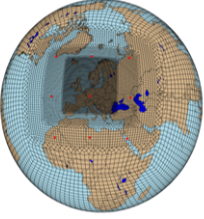
\includegraphics[height=4.5cm]{images/gg-a.png}
  \caption{Selected domains from our use cases. From left to right: interactive
    analysis of sea bass fish track reconstructions on biologging tag data (sea bass)
    with low resolution marine physics data; electron
    density of benzene molecule computed with Octopus; NorESM arctic grid for running Earth System Modelling experiments.
    (Background map: \copyright
    OpenStreetMap contributors ) \label{fig:applications}}
\end{figure}

\subsubsection{Open source ecosystem --- Jupyter and Binder}\label{sec:opensource}

The Binder Project \cite{binder} (\url{https://jupyter.org/binder}) is
a sub project of the Jupyter project, although it is not confined to be
useful only for notebooks, which are the focus of much of Jupyter.
\myemph{Project Jupyter} \cite{Jupyter}, which has grown increasingly popular in the scientific
computing community, has become the \emph{lingua franca} of interactive
computing in both academia and industry \cite{Perkel2018}. The main goal of Project Jupyter
is to provide a consistent set of tools to improve researchers'
workflows from the exploratory phase of the analysis to the communication
of the results \cite{Kluyver2016,Granger2021}.

The key components of the Binder tools are \repotodocker{}
(Section~\ref{sec:repo2docker}) and \binderhub{} (Section~\ref{sec:binderhub}). The \repotodocker{} tool
creates a \textbf{software environment} inside a Docker container from a \textbf{software
specification} in a \textbf{repository}. \binderhub{} starts a Jupyter notebook server
within this container from which the user can \textbf{execute} the notebooks or other scripts from the
repository.

The \emph{\mybinder{}} service (see \ref{sec:mybinder}) is provided by the \myemph{BinderHub
Federation} that collectively host a service running the Binder software
under the URL \url{https://mybinder.org}. (This is the service we made use of in the example
of Section~\ref{sec:reproducibility-example}.)

The BinderHub Federation is currently composed of three deployments of the BinderHub software

\begin{compactitem}
\item \url{https://gke.mybinder.org}, operated by the Binder team, and hosted on Google Cloud,
\item \url{https://ovh.mybinder.org}, operated and hosted by OVH,
\item \url{https://gesis.mybinder.org}, operated and hosted by GESIS.
\end{compactitem}

The focus for this proposal is to improve \repotodocker{}. In particular,
\repotodocker{} solves the software environment challenge (see
Section~\ref{sec:reproducibility-challenges}) in a generic way and is independent
from Jupyter notebooks.


\paragraph{\repotodocker}\label{sec:repo2docker}
The \repotodocker{} tool aims to \myemph{automate existing practices} for reproducible environment specification.
It looks in \textbf{repositories}, finds \emph{standard} \textbf{environment specifications} and produces \emph{typical} installation commands,
constructing a \textbf{software environment} in a Docker container image.
\repotodocker{} can fetch a remote repository and build a software
environment for this repository. Currently, \repotodocker{} can retrieve
repositories from at least the following services and formats: GitHub, Gist, GitLab, any git repository,
Zenodo, Hydroshare, Figshare, and Dataverse.

For the automatic building of reproducible computational environments,
\repotodocker{} understands commonly used conventions for environment specifications and
community standard tools such as Docker, conda, mamba, and pip.
The
documentation\footnote{\url{https://repo2docker.readthedocs.io/en/latest/config_files.html}}
  contains a full list.

\repotodocker{} is successful enough to be widely adopted,
but many shortcomings have been identified,
especially when a repository contains an \emph{incomplete} specification.
A common issue is to produce an environment that works when published,
but which may not produce a working environment at a later point in time,
due to version drift and insufficiently strict specifications.
Additionally, community practices not yet supported by \repotodocker{} have been proposed by their respective community members,
but the \repotodocker{} team has not had the funding support to incorporate and maintain them.

\paragraph{BinderHub}\label{sec:binderhub}
BinderHub is software for hosting a \textbf{web service} built on \repotodocker{} and
\JupyterHub{} where individuals can share \textbf{reproducible environments for
immediate and free interaction} by readers in their browser.

The BinderHub software exposes \repotodocker{} and Jupyter as a service,
allowing \textbf{one-click reproduction of published environments for interactive exploration}.
BinderHub is shown to work well,
but has limited application due to technical limitations,
such as its reliance on the Kubernetes deployment platform,
or challenges with combining the convenience of BinderHub's anonymous-by-default model
with authenticated and/or performant access to large data or compute resources.

While the \repotodocker{} terminal utility \emph{can} technically be used anywhere,
the technical expertise required is dramatically greater than a single click on a website such as mybinder.org.

\paragraph{Binder example}
\label{binder-how-does-it-work}

The most common reproducibility use case -- with the current state of the
\textbf{Binder tools} -- is the one we introduced in
Section~\ref{sec:reproducibility-example} using the \mybinder{} service. We will use this to
describe the role of the individual components of the Binder tools:

\begin{figure}[ht]
  \centering
    \includegraphics[width=0.7\textwidth]{images/mybinder.png}
    \caption{Home page of the \mybinder{} service.}
    \label{fig:mybinder-homepage}
\end{figure}

\begin{compactitem}
\item The \binderhub{} service is given a URL that encodes the location of the data
  repository\footnote{For example the
    {\url{https://mybinder.org/v2/gh/fangohr/reproducibility-repository-example/HEAD?labpath=figure1.ipynb}}
    refers to the GitHub repository ``reproducibility-repository-example'' of the
    github user ``fangohr'', asking to open the ``figure1.ipynb'' file.}
  (see Figure~\ref{fig:mybinder-homepage})
\item \binderhub{} will use
  \repotodocker{} to create a \textbf{software environment} (Docker image)
  in which the notebooks or scripts from the repository can be executed.
\item \repotodocker{} searches the repository for \textbf{software specifications}.
\item \repotodocker{} constructs the \textbf{software environment}
  from the \textbf{software specification(s)} (a Docker image).
\item \binderhub{} asks \JupyterHub to start
  a \textbf{notebook session} in this \textbf{software environment}.
\item \binderhub{} forwards the user who requested this environment to
  the URL at which the repository (or a particular notebook) can be
  \textbf{explored interactively} from within the Jupyter application.
\end{compactitem}

\paragraph{The \mybinder{} service}\label{sec:mybinder}

The \mybinder{} service is run by the BinderHub
Federation\footnote{\url{https://mybinder.readthedocs.io/en/latest/about/federation.html}}
of organisations. Collectively, they host a service running the BinderHub software
which can be reached from \url{https://mybinder.org}.
The service is \textbf{actively used} with approximately 200,000 sessions being
requested and delivered by the \mybinder{} service every week in 2021. The number
of sessions is growing from approximately 10,000 per day in November 2018
(beginning of the available records) to about \textbf{30,000 sessions per day} in 2022. We have
identified \textbf{60,000 unique repositories published} in the last few years which have
used the \mybinder{} service. The data is available~\cite{mybinder-archive}.

Examples of reproducible repositories that make use of the \mybinder{} service
include reproducible research repositories
\cite{GitHubRepoExampleAlbert2016,Beg2021}, interactive textbooks
\cite{Fangohr2022,Zeller2022} and citizen science and outreach activities
\cite{ligo-open-science,OSCOVIDA2022}.

This \TheProject{} project will not provide or operate a public BinderHub service such as the global
\mybinder{} instance. The resulting improvements to Binder tools, however, will be
immediately available for \textbf{exploitation by all operators of BinderHubs}, including \mybinder{}.


\subsubsection{Technical Readiness Level (TRL)}

Binder tools can be used in many ways, and their TRL depends on the context.
% TRL is unusual for Binder tools, because they are tools that can be used in many ways,
% and they can be described as having a different TRL \emph{in different contexts}.
The Binder software and service demonstration at mybinder.org is TRL 6,
where scope \emph{excludes} long-term robustness.
The Binder software for deploying services with authenticated access to data is TRL 3.
We will bring it to TRL 6.
The Binder tool repo2docker when targeting robust reproducible environments is TRL 4.
We will bring it to TRL 6.


\subsubsection{Community Engagement Panel}\label{sec:community-engagement-panel}
The Community Engagement Panel (CEP) is a forum we created for this project to bring together
representatives of \textbf{current and potential user communities} of Binder tools.
Through the community engagement panel, we aim to maximise the interaction between existing and new users.
This will help shape the software features so that we can
achieve the highest possible impact for practical reproducibility in science.
Stakeholders for the topic of reproducibility that should be represented in the
community engagement panel include \textbf{researchers, research infrastructure
providers, publishers, research councils, librarians, and educators}.

We have already secured agreement from the following to be part of the panel,
and will extend this if funded:
\begin{itemize}
\item Suzanne Dumouchel, Head of European Cooperation at TGIR Huma-Num CNRS unit, a large infrastructure for
digital humanities and member of the EOSC Association Board of Directors. She is the partnerships coordinator
of OPERAS Research Infrastructure, devoted to scholarly communication in Social Sciences and Humanities and is a member of DARIAH ERIC Coordination Office,
dedicated to Digital Arts and Humanities. She is also the scientific coordinator of TRIPLE, H2020 project
(INFRAEOSC2). Strongly committed to the Open Science movement and to the promotion of research in Social Sciences
and Humanities (SSH), she is particularly active in the field of research infrastructures.
\item Andy Götz, Software Group Leader at European Radiation Synchrotron
  Facility (ESRF), coordinator of the EOSC project PaNOSC for making data from
  photon and neutron facilities FAIR, and chairman of the IT working Group of
  the ``League of European Accelerator-based Photon Sources'' (LEAPS). The LEAPS
  facilities wish to enable their users to create reproducible publications
  based on large data sets captured at the light sources.
\item Paula Andrea Martinez, Project Coordinator - Software Program, \href{https://ardc.edu.au/}{Australian Research Data Commons} (ARDC).
She is also the co-chair of the \href{https://www.rd-alliance.org/groups/fair-research-software-fair4rs-wg}{FAIR4RS RDA Working Group} and
Community Manager at \href{https://www.researchsoft.org/}{Research Software Alliance} (ReSA), and actively contributing
to increase the visibility of research software.
\item Aleksandra Nenadic, Training Lead of the Software Sustainability Institute,
based at the University of Manchester (UK). She is also an active member and
promoter of the Carpentries community and involved as an instructor,
instructor trainer, mentor, workshop organiser and regional coordinator
for the UK, driving and supporting new material creation using the
Carpentries collaborative and pedagogical lesson development principles.
\item Gergely Sipos, head of services, solutions and support department at the
  EGI Foundation. He is representing EGI, ``Advanced Computing for EOSC''
  (EGI-ACE) and the EOSC Compute Platform, which are working on a large-scale
  deployment of BinderHub as part of their services for researchers in Europe
  and beyond.
\item Violaine Louvet, head of GRICAD (Grenoble Alpe Research -
 Scientific Computing and Data Infrastructure), supported by
 CNRS, Grenoble Alpes University and INRIA. GRICAD is a Tier 2
 infrastructure and provides data and computing resources to all the
 science communities in Grenoble. In particular, GRICAD provides HPC,
 HTC, cloud and storage resources for all the disciplinary fields,
 from computer sciences to human sciences and health. GRICAD
 also offers a JupyterHub and a BinderHub platform. We are also very
 involved in helping the scientific communities and in training activities.
 \item Rollin Thomas, Big Data Architect at HPC expert at the National Energy
  Research Scientific Computing Center at Lawrence Berkeley National Laboratory
  (US). He represents the HPC community, and focuses on interactivity,
  real-time, and reproducibility in supercomputing for science.
\item Andreas Zeller, Professor of Software Engineering at Saarland University. He uses Notebooks
  to provide open-source text books to his students and the world-wide
  community of readers. He will represent Binder users in academia, who use it
  to deliver zero-install computational environments for educational
  purposes.
\end{itemize}


\subsubsection{Gender aspects}\label{sec:gender}

\eucommentary{Describe how the gender dimension (i.e. sex and/or gender
  analysis) is taken into account in the project's research and innovation
  content [e.g. 1 page]. If you do not consider such a gender dimension to be
  relevant in your project, please provide a justification.}

\eucommentary{
	Note: This section is mandatory except for topics which have been identified
  in the work programme as not requiring the integration of the gender dimension
  into R\&I content.
}

\eucommentary{
	Remember that that this question relates to the content of the planned
  research and innovation activities, and not to gender balance in the teams in
  charge of carrying out the project.
}

\eucommentary{
	Sex and gender analysis refers to biological characteristics and
  social/cultural factors respectively. For guidance on methods of sex/gender
  analysis and the issues to be taken into account, please refer to
  \url{https://ec.europa.eu/info/news/gendered-innovations-2-2020-nov-24\_en}
}

\TheProject is committed to implement communication and outreach activities for
promoting the role of women and underrepresented groups in science
and STEM: i) present showcases to demonstrate the results of the project through
the eyes of underrepresented Research Software Engineers and researchers; ii)
systematically offer hybrid or online training opportunities to encompass the
lack of mobility of some potential attendees; iii) monitor gender participation
to our training, workshops, and hackathons and track progress. Members of the
consortium are involved in a number of programmes and activities who aim at
upskilling women and diversity and inclusion, for instance The Carpentries and
CodeRefinery training programmes and mentoring programs such as Outreachy or
Open Life Science.

Beyond outreach and communication, the Jupyter Project is committed to fostering an
inclusive and welcoming environment for everyone, and we will benefit from that
experience for example through a code of conduct for workshops and online events.

\subsubsection{National and international research or innovation activities}

\eucommentary{Describe any national or international research and innovation
  activities whose results will feed into the project, and how that link will be
  established; [e.g. 1 pages]}

The SOURCE project, as part of the overall Jupyter environment, will intrinsically build on the achievements of many
national and European and international research and innovative developments.
%which have been produced or are
% being implemented in research projects in which research infrastructures and project partners are or have been
% involved.
The Jupyter Project itself and its software ecosystem provides a substantial international
 research and innovation activity which will both feed into this project and benefit from it directly.
 Initial points of contact, beyond common ambitions to foster open science, are
 provided through the participants who have been long-time members of Project
 Jupyter (\site{SRL}, \site{QS}).

The science applications build on the outcomes of national, Nordic, European and/or international research and
innovation projects and initiatives. For example, both Ifremer and the University of Oslo are active members of the international
Pangeo\footnote{\url{https://pangeo.io/}} Big data Geosciences Community. Ifremer, through its co-ownership of Mercator Ocean International,\footnote{\url{https://www.mercator-ocean.eu/}}
 participates in the operation of the Copernicus Marine Environment Monitoring Service (CMEMS),
 a part of Copernicus, the European Union’s Earth Observation Programme and is also actively involved in the
 development of a Digital Twin of the Ocean that will be fully compatible with the Destination Earth (DestinE\footnote{\url{https://digital-strategy.ec.europa.eu/en/policies/destination-earth}})
 architecture and supports the European's Digital Strategy and Green Deal
 Package.
 See also Section~\ref{sec:science-applications} and
 Section~\ref{sec:consortium} for additional research activities.

\subsubsection{Interdisciplinarity}

\eucommentary{Explain how expertise and methods from different disciplines will be brought together and integrated in pursuit of your objectives. If you consider that an inter-disciplinary approach is unnecessary in the context of the proposed work, please provide a justification. [e.g. 1/2 page]
}
\TheProject{} brings together research software engineers with researchers from
multiple science domains to develop tools and methods that work across
scientific domains. An interdisciplinary approach is key to our success
(see Section~\ref{sec:complementarity-and-interdisciplinarity}).
In particular, we bring together core software engineers with expertise in developing and maintaining research software,
with researchers delivering cutting-edge research,
educators, and research infrastructure providers.
Each represents different stakeholders and expertise in the full lifecycle of reproducible research --- from tool development, to user needs, to service provider,
ensuring we have the best chance to solve real-world problems
with a lasting impact for better reproducibility in science.

\subsubsection{Open science practices and implementation}\label{sec:open-science-practices}

\TheProject will make use of open source licensed software, packages and
libraries, following the OSI
recommendations.\footnote{\url{https://opensource.org/licenses}}
All codes in this project will be open source and collaboratively developed using GitHub, following best software engineering practice
such as version control, tests, and continuous integration.
Training materials will be collaboratively developed through the {Carpentries
  Incubator}\footnote{\url{https://carpentries-incubator.org}}
using the {Carpentries Curriculum Development Handbook}:\footnote{\url{https://cdh.carpentries.org}} all Carpentries lessons are licensed under
the {Creative Commons Attribution version 4.0 (CC-BY)}\footnote{\url{https://creativecommons.org/licenses/by/4.0/legalcode}} and any related software under
the {MIT license}.\footnote{\url{https://opensource.org/licenses/MIT}}
All code will be developed fully in the open,
actively soliciting community engagement and transparency.

Use cases and showcases will only make use of data that are openly available.

All publications and/or any research data produced within \TheProject will be published Open Access.


\eucommentary{Describe how appropriate open science practices are implemented as
   an integral part of the proposed methodology. Show how the choice of practices
   and their implementation are adapted to the nature of your work, in a way that
   will increase the chances of the project delivering on its objectives [e.g. 1
   page].
%
   If you believe that none of these practices are appropriate for your
   project, please provide a justification here.
   }

\eucommentary{Open science is an approach based on open cooperative work and systematic
   sharing of knowledge and tools as early and widely as possible in the process.
   Open science practices include early and open sharing of research (for example
   through preregistration, registered reports, pre-prints, or crowd-sourcing);
   research output management; measures to ensure reproducibility of research
   outputs; providing open access to research outputs (such as publications,
   data, software, models, algorithms, and workflows); participation in open
   peer-review; and involving all relevant knowledge actors including citizens,
   civil society and end users in the co-creation of R\&I agendas and contents
   (such as citizen science).}

\eucommentary{Please note that this question does not refer to outreach actions that may be
   planned as part of communication, dissemination and exploitation activities.
These aspects should instead be described below under 'Impact'.}

\subsubsection{Research data management and management of other outputs}

The Data Management Plan (DMP) will be prepared and regularly updated within WP1.

Except for the software and usage data described below,
\TheProject activities will not generate or collect data.
While we have many demonstrators that interact with data, they do not generate or collect that
data themselves, but rather provide analytical mechanisms or access to data governed by
existing data management plans and data policies of project partners at each site,
as well as publicly accessible open data.

All data generated, collected, processed and stored will be made available following the
relevant standards and regulations. Processing of personal data in relation to training,
hackathons and/or workshop events will comply with GDPR regulations e.g. data
anonymisation and minimisation before sharing.
Procedures to monitor the real-time effectiveness of our dissemination and
communication strategies will also be GDPR compliant.
We have no plans to collect or produce personally identifiable information (PII)
during the project.\medskip

\paragraph*{Software}
Most research data from \TheProject will take the form of code.
All code produced by \TheProject will be developed in the public using open
source licenses (see Section~\ref{sec:open-science-practices}).
Milestone achievements of the software may be archived
in separate repositories such as Zenodo,
e.g. to coincide with publications.

\paragraph*{Service usage data}
Any data collected through the operation of public services
(e.g. popularity data for public open science repositories)
will be fully anonymised to the satisfaction of relevant best privacy practices and regulations, such as GDPR,
and made publicly available in the standard JSON Lines format,
as is done already for mybinder.org \cite{mybinder-archive}.
This is very small data and easily archived on free hosting services such as GitHub/Zenodo,
and will be made available under the Creative-Commons Universal Public Domain Dedication (CC0).
There is no cost to the project associated with archiving this data long-term.


\eucommentary{
Research data management and management of other research outputs: Applicants
generating/collecting data and/or other research outputs (except for
publications) during the project must provide maximum 1 page on how the data/
research outputs will be managed in line with the FAIR principles (Findable,
Accessible, Interoperable, Reusable), addressing the following (the description
should be specific to your project): [1 page]
}

\eucommentary{
Types of data/research outputs (e.g. experimental, observational, images, text,
numerical) and their estimated size; if applicable, combination with, and
provenance of, existing data.
}

\eucommentary{
Findability of data/research outputs: Types of persistent and unique identifiers
(e.g. digital object identifiers) and trusted repositories that will be used.
}

\eucommentary{
Accessibility of data/research outputs: IPR considerations and timeline for open
access (if open access not provided, explain why); provisions for access to
restricted data for verification purposes.
}

\eucommentary{
Interoperability of data/research outputs: Standards, formats and vocabularies
for data and metadata. Reusability of data/research outputs:  Licenses for data
sharing and re-use (e.g. Creative Commons, Open Data Commons); availability of
tools/software/models for data generation. }


%%% Local Variables:
%%% mode: latex
%%% TeX-master: "proposal"
%%% End:


% ---------------------------------------------------------------------------
%  Section 2: Impact
%  ---------------------------------------------------------------------------
\draftpage
% ---------------------------------------------------------------------------
%  Section 2: Impact
% ---------------------------------------------------------------------------

\clearpage
\section{Impact}
\label{sec:impact}

\subsection{Pathway toward impact}

\eucommentary{
e.g. 4 pages
Impact: Logical steps towards the achievement of the expected impacts of the project over time, in particular beyond the duration of a project. A pathway begins with the projects' results, to their dissemination, exploitation and communication, contributing to the expected outcomes in the work programme topic, and ultimately to the wider scientific, economic and societal impacts of the work programme destination.
}

\begin{draft}
{
\textcolor{red}
%\eucommentary{
Provide a narrative explaining how the project's results are expected to make a
difference in terms of impact, beyond the immediate scope and duration of the
project. The narrative should include the components below, tailored to your
project.

(a)	Describe the unique contribution your project results would make towards (1) the outcomes specified in this topic, and (2) the wider impacts, in the longer term, specified in the respective destinations in the work programme.
	Be specific, referring to the effects of your project, and not R\&I in general in this field.
	State the target groups that would benefit. Even if target groups are mentioned in general terms in the work programme, you should be specific here, breaking target groups into particular interest groups or segments of society relevant to this project.
	The outcomes and impacts of your project may:
  \begin{compactitem}


\item	Scientific, e.g. contributing to specific scientific advances, across and within disciplines, creating new knowledge, reinforcing scientific equipment and instruments,  computing systems (i.e. research infrastructures);
\item	Economic/technological, e.g. bringing new products, services, business processes to the market, increasing efficiency, decreasing costs, increasing profits, contributing to standards’ setting,  etc.
\item	Societal , e.g. decreasing CO2 emissions, decreasing avoidable mortality,
improving policies and decision making, raising consumer awareness.
\end{compactitem}
Only include such outcomes and impacts where your project would make a
significant and direct contribution. Avoid describing very tenuous links to
wider impacts. However, include any potential negative environmental outcome or
impact of the project including when expected results are brought at scale (such
as at commercial level). Where relevant, explain how the potential harm can be
managed.

(b)	Describe any requirements and potential barriers - arising from factors beyond the scope and duration of the project - that may determine whether the desired outcomes and impacts are achieved. These may include, for example, other R\&I work within and beyond Horizon Europe; regulatory environment; targeted markets; user behaviour. Indicate if these factors might evolve over time. Describe any mitigating measures you propose, within or beyond your project, that could be needed should your assumptions prove to be wrong, or to address identified barriers.
	Note that this does not include the critical risks inherent to the management
  of the project itself , which should be described below under
  ‘Implementation’.

(c)	 Give an indication of the scale and significance of the project’s contribution to the expected outcomes and impacts, should the project be successful.  Provide quantified estimates where possible and meaningful.
	‘Scale’ refers to how widespread the outcomes and impacts are likely to be. For example, in terms of the size of the target group, or the proportion of that group, that should benefit over time; ‘Significance’ refers to the importance, or value, of those benefits. For example, number of additional healthy life years; efficiency savings in energy supply.
	Explain your baselines, benchmarks and assumptions used for those estimates. Wherever possible, quantify your estimation of the effects that you expect from your project. Explain assumptions that you make, referring for example to any relevant studies or statistics. Where appropriate, try to use only one methodology for calculating your estimates: not different methodologies for each partner, region or country (the extrapolation should preferably be prepared by one partner).
	Your estimate must relate to this project only - the effect of other initiatives should not be taken into account.
}
\end{draft}


Almost all researchers perform some kind of computation in the course of their work,
from production of simple charts and figures to large-scale simulations.
Researchers today are faced with a great variety of useful
and increasingly open tools to perform their research tasks.
However, this variety presents its own challenge.
Because we are building and extending \textbf{generic tools for computational reproducibility},
we help researchers of all kinds perform their work reproducibly without dictating
how they do the research part of their work.
By focusing on (\textbf{reproducible computational environments}),
and offering a generic and interoperable solution,
we \emph{are} solving a big piece of the reproducibility problem
and act as a bridge between any solutions to other parts of the reproducibility problem,
for instance those classically addressed by workflow management systems.
"Do one thing and do it well" is key to success and will accelerate progress
by allowing others to concentrate on different challenges in the reproducibility problem.

Helping researchers navigate this diverse landscape of research software
with both education and practical tools
will enable a \textbf{large fraction of all researchers to perform research in a more efficient,
more productive, more reproducible, and more \emph{useful} way}.

\subsubsection{Contributions towards outcomes and impact}
\label{sec:countributions-towards-outcome-and-impact}

The expected outputs and impact of \TheProject with respect to the
work program is detailed in Tables~\ref{table:output-comparison}
and~\ref{table:impact-comparison}, respectively.

%\begin{table}[p]
\begin{table}[h!]
  \begin{center}
    \begin{tabular}{>{\raggedright}m{.30\textwidth}|m{.65\textwidth}}
      \toprule
      \textbf{Expected outputs from call}
      & \textbf{Expected outputs from the \TheProject project}\\\midrule
        %
        %
      Structured understanding of the underlying drivers, of concrete and effective
      interventions -- funding, community-based, technical and policy -- to increase
      reproducibility of the results of R\&I; and of their benefits;
      &
      %
        Developing a structured understanding of the technological challenges of practical
        reproducibility of software environments is a prerequisite for our work on the
        community-effort-based Binder tools (\WPref{reproducibility}, \WPref{impact},  \WPref{applications}).

        We know that the technologies such as the Jupyter notebook and their reproducibility
        with Binder find some acceptance in the scientist community (see Section~\ref{sec:opensource}).
        One of the outcomes of this project is an improved structured understanding of the underlying drivers
        for the wider research community to adopt or not adopt these technologies as a concrete and effective action to improve the reproducibility of their results~(\WPref{education}). We expect an interplay of technical, social, community-specific and policy drivers affecting this.
        %
      \\\midrule
      Effective solutions, policy-, technical- and practice-based, to increase the
      reproducibility of R\&I results in funding programmes, in communities and in
      the dissemination of scientific results;
      &
        The Binder tools are effective and practice-based technical solutions to increase the
        reproducibility of R\&I results in funding programmes and in scientific research more widely~\cite{Beg2021}.
        The combination of Jupyter notebooks and Binder are also effective solutions for the dissemination through
        workshops~\cite{binder-workshops} and education activities~\cite{Zeller2022} involving computation as participants can use complex
        software environments through their browser, and do not need to install any additional software locally.
      \\\midrule
      Greater collaboration, alignment of practices and joint action by stakeholders
      to increase reproducibility, including but not limited to training,
      specialised careers and guidelines for best practice.
      &
        \TheProject is developing tools that enable \textbf{automatic computational reproducibility} across many domains by aligning to the existing software specification practices. Having one tool that respects existing practices means it can be adopted across many domains, thus \textbf{facilitating greater collaboration}. We will develop \textbf{best practice guidelines} for reproducibility and open science, and disseminate them through training activities and materials. The staff hired for the project will be highly specialised research software engineers. We expect that voluntary contributors attracted by the project will also receive additional training for such specialised careers.
      \\\bottomrule
    \end{tabular}
  \end{center}
  \caption{Relating \TheProject outputs to the outputs expected by the call \label{table:output-comparison}}
\end{table}


\begin{table}[h!]
  \begin{center}
      \begin{tabular}{>{\raggedright}m{.2\textwidth}|m{.75\textwidth}}
      \toprule
      \textbf{Expected impacts from call}
      & \textbf{Expected impacts from the \TheProject project}\\\midrule
        %
        %
      Increased proportion of reproducible results from publicly funded R\&I
      &
      %
        The \TheProject project will improve the ease of use tools for reproducibility,
        thereby \textbf{increasing the number of reproducible research outputs}.
        The project will also \textbf{educate researchers} to provide the motivation, required
        technical skills, and an understanding of best practice to achieve
        reproducible science outcomes.
      \\\midrule

        %
        %
      Increased re-use of scientific results by research and innovation
      &
        \textbf{Reproducibility enables reusability}, in particular where the reproduction
        of the results can be carried out automatically (for example using the
        tools developed and improved in the \TheProject project).

        From anecdotal evidence, it is known that
        a new PhD student may need many months (sometimes exceeding 12 months) to reproduce
        a published study which is to form the basis of their new research task.
        An immediately reproducible research output made available together with the publication
        can reduce this time immensely: a binder-enabled reproducible repository may be able
        to recompute the results within an hour or a much shorter time because the process is automatic.

        The availability of an immediately reproducible research output -- as fostered by \TheProject{} -- plays a very
        important role in modern research, where generally advances are built based on prior results.\\\midrule

      Greater quality of the scientific production.
      &
        %Reproducibility is an important concept underpinning the scientific method.
        %Re-usability of results -- often enabled through their reproducibility -- has the potential to accelerate the research significantly.

        The availability of practical reproducibility as advanced by \TheProject has the potential to
        improve the quality of scientific research through new opportunities for collaboration and interdisciplinary research:

        We have already seen a good example of the Jupyter ecosystem facilitating an
        interdisciplinary collaboration: the Nobel Prize-winning LIGO scientific collaboration shared
        notebooks detailing the data processing steps which led to the discovery of
        gravitational waves, using the Binder service to allow anyone to re-compute
        the published plots~\cite{ligo-open-science}. Scientists with no background in gravitational waves
        studied these notebooks and improved the signal processing.

        In this proposal, we want to provide this ability to a wider audience through
        improved tools and documentation,
        including for disciplines which rely on processing much larger volumes of
        data.\\
      \bottomrule
    \end{tabular}
  \end{center}
  \caption{Relating \TheProject impacts to the impacts expected by the call \label{table:impact-comparison}}
\end{table}

%\newpage
\subsubsection{Measuring impact}\label{sec:KPIs}

As we are building tools for open and reproducible science, the best measure of our impact
is in the adoption and use of these tools and services based on them. This can be observed
qualitatively (anecdotal feedback and case studies) and quantitatively (counting workshop
attendees, for example).
%
% Much of our work will be in the form of contributions to existing
% public projects, such as Binder and Jupyter, which can be measured in our participation in
% those projects, such as code and documentation contributions, bug reports, and roadmap
% contributions.
%
We measure progress toward our objectives (Table~\ref{tab:objectives-tasks})
via the following Key Performance Indicators (KPIs):
\begin{compactenum}[\textbf{KPI} 1:]
\item \label{kpi:reproducibility} Fraction of published repositories for
  which Binder tools can build the computational environment -- measuring both
  improvements in Binder tools and impact from our training efforts. We will
  implement the required methodology in
  \taskref{reproducibility}{repo2docker-checker}. (Objective 1)
    % Open publications for which the authors have made a reproducible repository available
    % through \TheProject services.
\item \label{kpi:broaden} Number of researchers who benefit from using
  \TheProject{} results in their work. Due to the open source nature of our
  outcomes, it is difficult to track this number accurately. To solicit this
  information, we can request feedback from users on forums, mailing lists and
  social media, and count the users we know directly working with
  them through \WPref{applications} and \WPref{education} for example. We expect
  to under count beneficiaries for this metric, but believe the KPI is still useful
  to measure our direct impact for better reproducibility in science. (Objective 2)
\item \label{kpi:demonstrators} Number of demonstrators enabled that make
  results from scientific research reproducible. (Objective 3)
\item \label{kpi:education} Metrics to capture the number of people that have
  made use of the training and education activities of \TheProject{}, such as
  workshop attendees, viewers of training videos, access to online documentation
  of best practice. (Objective 4)% can we track people accessing a documentation web site?
\end{compactenum}


\subsubsection{Target groups and scale of impact}\label{sec:target-groups-and-scale-of-impact}

We have already discussed in Section~\ref{sec:motivation-why} that
\textbf{computational reproducibility affects the majority of researchers},
including those who carry out work that is not predominantly computational.

The impact of this project will be realised through (i) the training we develop
and disseminate, and (ii) the improved Binder tools. The improved tools will
directly impact the community of researchers using Jupyter notebooks. However,
the \myemph{improved functionality and applicability of the Binder tools outside Project
Jupyter} will benefit all researchers who need computational reproducibility, and
may be -- and in the long run -- more important.

\medskip

We can give some indication of the size and activity of the Jupyter notebook
community and use of the existing Binder tools: Jupyter notebooks are used to
support research in numerous communities, including
%\begin{compactitem}
%\item
\noemph{Journalists} and practitioners of \noemph{data-driven
journalism} at the LA Times, BuzzFeed News, Columbia Journalism School
\cite{latimes-datadesk} \cite{columbia-nytimes} \cite{data-journalism};
\noemph{Data scientists} in academia, industry and services \cite{Perkel2018};
% \item
\noemph{Research institutions} such as CERN, EuXFEL, JRC, and many more,
operating institution-wide Jupyter deployment;
% \item
\noemph{Universities} using Jupyter as a teaching platform;
% \item
\noemph{Large cloud providers} building commercial products on the
top of Jupyter (Google DataLab and Colaboratory, AWS Sagemaker, OVH AI Notebook);
% \item
within the \noemph{European Open Science Cloud}, Jupyter is used in many EOSC
projects, and a JupyterHub service is provided by the EGI foundation.
% \item
This impact was recognised by the \emph{ACM Software System Award} that was
awarded to the Jupyter team to honour \emph{"developing a software system that
had a lasting influence"} in 2017. (Prior recipients include \emph{Unix},
\emph{TCP/IP}, and the \emph{World Wide Web} \cite{acm-award}.)

There are \textbf{at least 8 million notebooks} deposited on GitHub \cite{notebookcount}, and
the size of the \textbf{notebook user base was estimated} to be of the order of
\textbf{millions in 2015} \cite{jupyter-grant}. We know that the public Binder service \textbf{\mybinder{}
was used to create over 10,000,000 computational environments}
from at least 50,000 unique repositories in 2021~(Section~\ref{sec:opensource}).


\subsubsection{Potential barriers}

A central barrier towards impact would be if the research community would not
accept or embrace the tools and practical guidance developed here.
To minimise this risk, we'll stay in close touch with all our stakeholders
(\WPref{management}, \WPref{applications}, \WPref{education}), and use
the experience of the team members who are active researchers themselves.

A key strategy in mitigating barriers to adoption is the approach of \textbf{automating existing practices}.
All of the \textbf{practices promoted} and developed by \TheProject \textbf{are beneficial} to
producers and consumers of reproducible research alike,
\textbf{independent of the specific Binder tools} in which we choose to implement the automation.
This avoids lock-in and ensures positive impact even among researchers who choose not to use any of the specific tools we develop.

\subsection{Measures to maximise impact -- dissemination, exploitation and communication}

\eucommentary{
e.g. 5 pages, including 2.3
}

\begin{draft}
  \textcolor{red}
Describe the planned measures to maximise the impact of your project by providing a first version of your ‘plan for the dissemination and exploitation including communication activities’. Describe the dissemination, exploitation and communication measures that are planned, and the target group(s) addressed (e.g. scientific community, end users, financial actors, public at large).

Please remember that this plan is an admissibility condition, unless the work programme topic explicitly states otherwise. In case your proposal is selected for funding, a more detailed ‘plan for dissemination and exploitation including communication activities’ will need to be provided as a mandatory project deliverable within 6 months after signature date. This plan shall be periodically updated in alignment with the project’s progress.

Communication measures should promote the project throughout the full lifespan of the project. The aim is to inform and reach out to society and show the activities performed, and the use and the benefits the project will have for citizens. Activities must be strategically planned, with clear objectives, start at the outset and continue through the lifetime of the project. The description of the communication activities needs to state the main messages as well as the tools and channels that will be used to reach out to each of the chosen target groups.

All measures should be proportionate to the scale of the project, and should contain concrete actions to be implemented both during and after the end of the project, e.g. standardisation activities. Your plan should give due consideration to the possible follow-up of your project, once it is finished. In the justification, explain why each measure chosen is best suited to reach the target group addressed. Where relevant, and for innovation actions, in particular, describe the measures for a plausible path to commercialise the innovations.

If exploitation is expected primarily in non-associated third countries, justify by explaining how that exploitation is still in the Union’s interest.

Describe possible feedback to policy measures generated by the project that will
contribute to designing, monitoring, reviewing and rectifying (if necessary)
existing policy and programmatic measures or shaping and supporting the
implementation of new policy initiatives and decisions.
\begin{compactitem}
\item	Outline your strategy for the management of intellectual property, foreseen protection measures, such as patents, design rights, copyright, trade secrets, etc., and how these would be used to support exploitation.
	If your project is selected, you will need an appropriate consortium agreement
  to manage (amongst other things) the ownership and access to key knowledge
  (IPR, research data etc.). Where relevant, these will allow you, collectively
  and individually, to pursue market opportunities arising from the project.
\item If your project is selected, you must indicate the owner(s) of the results (results ownership list) in the final periodic report.
\end{compactitem}
\end{draft}


\TheProject is contributing to tools for open and reproducible science. It is
essential that we disseminate our work in order to \textbf{reach and support user
communities} (such as researchers and research infrastructure providers), enable
them to best exploit our software and services, and achieve impact.
This section outlines how the project will establish and organise the
dissemination, communication, and exploitation actions to promote the project
and the adoption of its outcomes beyond the project's lifetime.


% The dissemination and communication plan is outlined in the following sub-sections.
% Therein we distinguish:
% \begin{itemize}
% \item Dissemination as the public disclosure of the results of the project through
% a process of promotion and awareness-raising right from the beginning of a project.
% It makes research results known to various stakeholder groups (like research peers, industry
% and other commercial actors, professional organisations, policymakers) in a targeted
% way, to enable them to use the results in their own work.
% \item Communication as the strategic and targeted measures for promoting the project
% and its results to a multitude of audiences, including the media and the public, and possibly
% engaging in a two-way exchange. The aim is to reach out to society as a whole and
% in particular to some specific audiences while demonstrating how EU funding contributes to tackling
% societal challenges.
% \end{itemize}

\subsubsection{Dissemination of results}

\TheProject endeavours to make open and reproducible science practices both more \textbf{understandable and actionable}
to practitioners through the development and use of open and freely available tools.
Most of \TheProject software will be in the form of contributions to existing projects,
which will be governed by the licenses of those projects.
All Jupyter and Binder software is released under the permissive BSD license,
which specifically allows commercial exploitation,
as has proven successful in enabling collaborations with industrial partners
such as Google, Microsoft, IBM, OVHCloud, and more.
Any other developments will be made publicly and freely available under open source licenses, and
hosted on public code hosting sites such as GitHub.
This means that all \textbf{\TheProject software will be available and accessible to all} who find it,
at no cost to \TheProject,
enabling long-term access beyond the funding of \TheProject.
Similarly, non-code products such as dissemination works
(workshop materials, etc.) will be made freely available under open Creative Commons licenses.

All the partners will be involved in the dissemination of \TheProject results (see draft plan of the
dissemination, communication and exploitation plan in the text box in Section~\ref{box:draft-C-D-E-plan}) and
\WPref{applications} and \WPref{education} will play a central role.

As a result, the primary dissemination effort is to:
\begin{enumerate}
  \item make sure that \textbf{prospective users are aware of the work} through
    {show cases, science demonstrators, demos, best practice
      documentation, project communication}, and
  \item \textbf{enable them to use and exploit the tools} through learning resources, training, and services.
\end{enumerate}

Our focus for dissemination will be on
\taskref{education}{workshops}
operating workshops, training various communities in the availability,
purpose, development, and use of \TheProject software and services.
We will make a particular effort to use these workshops as an opportunity
to \textbf{support diversity and inclusion in the open science community},
by running (online, hybrid, or in-person) workshops for under-served and under-represented groups in the academic and
open source communities. \textbf{Free and online training} will be streamed (e.g. Twitch),
made available to the wider community for instance on YouTube, and archived on Zenodo for long-term availability and
findability to the wider community who may not be able to attend workshops.


These resources will be hosted on free, public hosting services,
such as GitHub Pages, ReadTheDocs, or YouTube channels, and as much as possible co-developed and co-hosted with existing and
well-established organisations
(The Carpentries,\footnote{\url{https://carpentries.org/}} CodeRefinery,\footnote{\url{https://coderefinery.org/}}
Galaxy Training Network,\footnote{\url{https://training.galaxyproject.org/}} Pangeo,\footnote{\url{http://gallery.pangeo.io/}} etc.).

We will also disseminate our results through \textbf{publications and conferences}.
All publications funded by \TheProject will be \textbf{open access},
and sites expecting publications have budgeted funds for paying open access fees.
We will identify and attend appropriate conferences for disseminating our work,
including running tutorials at conferences in historically interested communities such as PyData and SciPy.
Also, we will identify and attend conferences from complementary communities such as ROpenSci,
Mozilla Science, and Julia,
as well as domain specific conferences to maximise the impact of \TheProject and to broaden its
audience outside the
traditionally included communities.

The \textbf{operation of prototype services} in \WPref{applications} is also a dissemination activity,
as services like Binder not only enable open and reproducible science by facilitating interactive publications,
they also enable \textbf{interactive demonstration of tools and functionality}
developed in \TheProject.

\TheProject will also actively seek \textbf{collaboration} (through the Community
Engagement Panel and
\TheProject partners) with existing \textbf{EOSC projects} (many already use/deploy
Jupyter notebook services) to inform and support them in exploiting \TheProject
developments and adapting their service offerings.
\subsubsection{Exploitation}

Our primary outputs are in the form of software tools, prototype services, and information resources,
all of which will be freely available to all under appropriate permissive open
licenses (such as BSD/MIT).
This means that exploitation generally has the form of:

\begin{enumerate}
  \item Use of Binder tools for \textbf{producing reproducible environments} in research, as enabled by \WPref{reproducibility}
  \item Use of Binder tools for \textbf{evaluating reproducible environments} in research or publication \textbf{policy}, as enabled by \WPref{reproducibility}
  \item Use of Binder tools in the \textbf{construction and operation of services}, as enabled by \WPref{impact}
  \item Deploying \textbf{new services} derived from our science demonstrators in \WPref{applications}
  \item \textbf{Application of effective practices for reproducibility}, developed and disseminated in \WPref{education}
  \item \textbf{Commercial exploitation} via product development and consulting.
\end{enumerate}

A key aspect of our exploitation strategy is to focus our work on existing,
active projects in Binder and the wider Jupyter ecosystem.
This means that our contributions are of \textbf{immediate practical benefit to between
  thousands and millions of users} worldwide (Section~\ref{sec:target-groups-and-scale-of-impact}).

\TheProject contributions to Binder tools will be immediately (\emph{i.e.
  already during the duration of the project}) \textbf{exploited via the public mybinder.org service}
and its thousands of daily users (Section~\ref{sec:mybinder}), as well as \textbf{many BinderHub instances worldwide}.

The science demonstrators in \WPref{applications} are themselves exploitations of the outputs
in \WPref{reproducibility} and \WPref{impact},
building services not possible before the project.
\textbf{Continued operation and adoption of} these \textbf{reproducibility services} by project partners and the researchers they serve beyond
the duration of the project is anticipated for a majority of the science applications, and will indicate
successful exploitation of the project.

%\TOWRITE{ALL}{Specific per-site exploitation?}  Not needed I think - we have
%the demonstrators clearly mentioned.

The \site{QS} SME provides \textbf{commercial support and development services around the
open-source} scientific computing ecosystem. The team has specialised in the Jupyter ecosystem
and package management solutions, which are both at the core of this proposal. The consolidation
of Binder's technical foundations will help QuantStack provide robust solutions to its clients.

Industrial use cases met by QuantStack also show that the reproducibility issues addressed in this proposal go
beyond the scientific use case:

\begin{compactitem}
\item For example, \textbf{financial institutions} using numerical libraries to price and hedge derivatives must be able
   to reproduce results obtained with past versions of their software, especially in cases of mispricing or
   mishedging. Rolling back to a state of the software environment as of several years earlier may prove
   extremely difficult. Adopting the approach of Binder to favour reproducibility has proven to be a viable way
   to address this issue.
\item Similarly, in the field of \textbf{industrial robotics}, QuantStack has developed a conda-based distribution of the
   ROS open-source ecosystem called RoboStack, and a tool akin to repo2docker to produce container images providing
   all required packages for a ROS node, that will directly benefit from this work.
\end {compactitem}

This shows that techniques and software tools that arise from the computational
research communities to address reproducibility
will help address the same issue for a much broader audience, including commercial applications.

\subsubsection{Communication activities}

The main goals of the communication activities is making sure that researchers
and potential users are aware of the outputs, tools and services developed by \TheProject
on an ongoing basis, and to demonstrate to the public the clear benefits of the work they have funded.

In order to maximise this impact, it is vital to address the audience as one project
and ensure the immediate recognition of information stemming from it.
Together with all partners involved, \TheProject will therefore build a \textbf{strong project identity}
(see draft of the communication, dissemination, and exploitation plan in Section~\ref{box:draft-C-D-E-plan}) to strengthen the project
identity and to deliver clear messages to our audiences.

We will operate a \textbf{website}
(\taskref{management}{website}) for collecting and sharing information about \TheProject and its progress.
It will provide a centralised way to access the various publicly available deliverables, publications
and articles related to the project. The site will be regularly updated over the lifetime of the project
with the project publications and public materials, such as flyers, posters and
public deliverables, organised workshops, available services, news, etc.
Site analytics will be associated with the project website, in order
to provide useful insight on how to improve its impact. In addition, the project intends to
develop its presence on \textbf{the social and content
networks}. The channels will be used for interaction
with the professional community as well as the general public
(differentiation on the content per channel based on the target group wishing to address).
As part of the project's communication plan, \TheProject will develop a social media strategy
in order to increase outreach and social impact, which can be summarised as follows: (a) identifying target
audience and key stakeholders, (b) updating social media content and sparking
discussion in social media/tweeting, (c) measuring social impact and reassessing
social media strategy as required.

\subsubsection{Communication, dissemination, and exploitation plan}

We will continually refine our Communication, Dissemination, and Exploitation plans, starting with the draft below:
\label{box:draft-C-D-E-plan}
\begin{framed}

  \centerline{\textbf{ \TheProject DRAFT COMMUNICATION, DISSEMINATION, and EXPLOITATION}}
  {
  \begin{itemize}

\item Logo creation, standard document templates for deliverables, reports, letters, presentations, project posters/leaflets, etc. and creation and/or use of relevant social media accounts such as Linkedin, Twitter, YouTube channel (80k Twitter followers for @ProjectJupyter, 34k for @IPythonDev, and 132k for the PyData Youtube channel);
\item Annual plan for publication in scientific and technical peer-reviewed journals and conference proceedings;
\item Creation of \TheProject website:
\begin{itemize}
\item links to \TheProject repository of results (videos, training material, use cases, demonstrators, software and associated documentation such as repo2docker, JupyterJub and Binder);
\item links to social media accounts, e.g. on Facebook, Instagram, LinkedIn and Twitter and public communication channel (Zulip);
\item live “Infoboard” to highlight news and outcomes, event calendar, public resources, specific social media posts; This infoBoard will be relayed by the News (and Newsletter) of partnered projects (Jupyter, Pangeo, Ifremer, NeIC, Sigma2, etc.).
\item links to the EOSC catalogues of services and national/institutional
  services using and supporting \TheProject{} tools and outcomes;
\end{itemize}
\item Use the Community Engagement Panel to review the target audience for dissemination (workshops, training, hackathon, etc.), create a live list of communication partners and associated channels and tools;
\item Coordinate (annually) with other initiatives (The Carpentries, CodeRefinery, Jupyter, Pangeo) for the collaborative development of training material and the delivery of demos, training/workshops/hackathons;
\item Refine measurable goals (based on inputs/feedback from the Community
  Engagement Panel), quantitative KPIs for dissemination and monitoring procedures;
\item Develop and maintain a live collaboration plan for links and interactions with other projects (EC-funded, Nordic and/or national projects), research institutions and industries to find opportunities to show-case \TheProject results;
\item Develop a consolidated exploitation plan to ensure the long term and sustainable exploitation of the project results beyond its lifetime, in particular the deployment of EOSC services.
    \end{itemize}
}
\end{framed}

\clearpage
\subsection{Summary}

\eucommentary{
Provide a summary of this section by presenting in the canvas below the
key elements of your project impact pathway and of the measures to
maximise its impact.
KEY ELEMENT OF THE IMPACT SECTION
}

% measured original color as 0, 0.75, 0.95
% but it's a bit low-contrast

\definecolor{summaryblue}{rgb}{0, 0.7, 0.9}
\newtcolorbox{summarybox}[1]{
    colback=white,
    colframe=summaryblue,
    fonttitle=\bfseries,
    title={#1}
}

\begin{multicols}{2}

\begin{summarybox}{SPECIFIC NEEDS}
\eucommentary{What are the specific needs that triggered this project?}

Computational reproducibility is a widely recognised challenge. \textbf{Most
researchers need computational reproducibility} to achieve reproducible science
outcomes, such as publications.

There are many tools that solve \emph{part} of the problem,
or aim to solve the whole problem while requiring wholesale adoption of a specific tool.
This may not be practical or desirable across a variety of domains or
communities.

Additionally, \textbf{solving software environments is hard},
and researchers need easy-to-use \textbf{tools} to help.
\end{summarybox}

\begin{summarybox}{EXPECTED RESULTS}
\eucommentary{What do you expect to generate by the end of the project? }

\textbf{Improved software tools for reproducing computational environments}:
by improving the Binder tools for reproducible environments,
it will be easy for researchers to produce and share results openly and reproducibly.

\textbf{Improved understanding of good practices for reproducibility}: study results, documentation, and workshops will aid researchers and policy makers in understanding the most appropriate practices to adopt in their pursuit of reproducible research.

\end{summarybox}
\begin{summarybox}{D \& E \& C MEASURES}
\eucommentary{What dissemination, exploitation and communication measures will you apply to the results?}

\textbf{Exploitation:} We contribute to the \textbf{Binder tools},
already widely used by \TheProject members and hundreds of thousands world-wide.
All existing applications, from the \mybinder service to individual users,
immediately and directly benefit from our improvements to the tools.
Our science applications specifically exploit new features developed by the project.

The QuantStack SME will \textbf{commercially exploit} the improved Binder tools in areas ranging from
industrial robotics to quantitative finance.

\end{summarybox}

\begin{summarybox}{D \& E \& C MEASURES}
\textbf{Dissemination:} Results, insights, tools, and guidelines will
  be disseminated to potential users and stakeholders through conventional
  academic channels, in-person and remote workshops, websites, video tutorials
  and social media.

\end{summarybox}

\begin{summarybox}{D \& E \& C MEASURES}
\textbf{Communication:} The media and general public will be informed
  about the project through news releases, videos, a website, social media,
  further media engagement, flyers and interviews, with a consistent visual
  identity.
\end{summarybox}

\begin{summarybox}{TARGET GROUPS}
\eucommentary{Who will use or further up-take the results of the project? Who will benefit from the results of the project?}

\textbf{Computational science practitioners}: researchers with an interest in reproducibility of their own work.

\textbf{Research infrastructure providers}: organisations supporting researchers
through experimental and computational services.

\textbf{Research institutions}: institutions facilitating or enforcing the reproducibility of their researchers.

\textbf{Policy makers and publishers}: Funders and institutions requiring their subjects to follow reproducible practices.
\end{summarybox}

\begin{summarybox}{OUTCOMES}
\eucommentary{What change do you expect to see after successful dissemination and exploitation of project results to the target group(s)?}

\textbf{Adoption of Binder tools for reproducibility}:
practitioners will have access to Binder tools for reproducibility,
having improved their usability and robustness.

\textbf{Resources for reproducible practices}:
practitioners will have access to resources to learn about effective reproducibility practices.

\textbf{Facilitating practical policies for reproducible publications}:
policies will have access to tools for validating reproducible practices that they require.
\end{summarybox}

\begin{summarybox}{IMPACTS}
\eucommentary{
What are the expected wider scientific, economic and societal effects of the project contributing to the expected impacts outlined in the respective destination in the work programme?
}

\textbf{Improved reproducibility of scientific results}: Improving the \emph{ease of use} tools for reproducibility
lowers the barrier for adoption, and thereby increases the number, quality, and
access of reproducible research outputs, as well as increasing public trust in science.

\textbf{Increased re-use of scientific results}: Practical reproducibility
enables rapid re-use of published results leading to more effective research activities.

\textbf{Democratised science} by lowering the barrier to participation in the research process
and reproduction of scientific results.

\end{summarybox}
\end{multicols}
\clearpage

% \noindent
% \fbox{
% \begin{minipage}{
% % \dimexpr\linewidth-2\fboxrule-2\fboxsep
% 2in
% }
% \textbf{SPECIFIC NEEDS 2}
%
% xyz
% \begin{compactenum}
% \item x
% \item y
% \end{compactenum}
% \end{minipage}
% }
% {
% \hfill\makebox[0pt]{\fbox{
% \textbf{SPECIFIC NEEDS}}}
% \hfill
% }

% \textbf{SPECIFIC NEEDS}
%
% xyz
% \begin{compactenum}
% \item x
% \item y
% \end{compactenum}




%%% Local Variables:
%%% mode: latex
%%% TeX-master: "proposal"
%%% End:

\draftpage

% ---------------------------------------------------------------------------
%  Section 3: Implementation
% ---------------------------------------------------------------------------

\section{Quality and efficiency of the implementation}
\COMMENT{Typical granularity: 5-8 work packages with 3-5 tasks and one
  deliverable per task; 10 milestones}

\subsection{Work Plan and resources}

\label{sect:workplan}

\eucommentary{Please provide the following:\\
\begin{compactitem}
\item
brief presentation of the overall structure of the work plan;
\item
timing of the different work packages and their components (Gantt chart or similar);
\item
detailed work description, i.e.:
\begin{compactitem}
\item
a description of each work package (table 3.1a);
\item
a list of work packages (table 3.1b);
\item
a list of major deliverables (table 3.1c);
\end{compactitem}
\item
graphical presentation of the components showing how they inter-relate (Pert chart or similar).
\end{compactitem}
}

\subsubsection{Quality and efficiency of the implementation}\label{sec:workplan-structure}

\ifgrantagreement The \else As shown in Table~\ref{fig:wplist} and
Figure~\ref{fig:workpackages}, the \fi work plan is broken down into five work
packages: \WPref{reproducibility} focuses on robustness improvements of the
Binder tools, \WPref{impact} is advancing the Binder tools feature set to
increase the impact of the tools and project, \WPref{applications} applies and
evaluates the reproducibility tools in real-world research contexts.
\WPref{education} is focused on engaging with and educating researchers and the
wider public in best practices for reproducible science. This is complemented by
the usual management work package (\WPref{management}).

\begin{figure}[htb]
  \centering
  \includegraphics[width=0.67\textwidth]{images/WP.pdf}
  \caption{
    \label{fig:workpackages}
    The relationships and interactions of the work packages,
    broken up into four categories: Management (WP1),
    Development of new functionality surrounding Jupyter's Binder tools to improving robustness
    and Broadening impact (WP2, WP3),
    Applications of tools developed in real world research context (WP4),
    and Dissemination, education, and engagement (WP5: Dis., edu., eng.).
  }
\end{figure}

% \subsubsection{How the Work Packages will Achieve the Project Objectives}
% \label{sssec:how_the_work_packages_will_achieve}

\pagebreak The Gantt chart in
Figure~\ref{fig:gantt} %on page~\pageref{fig:gantt}
illustrates the distribution of time across the work packages over time.
The height of grey bars corresponds to total person month effort per
month for each work packages. We ramp up overall activity during year 1, then remain
at a constant level. In the beginning of the project, the work on core parts of
the technology dominates (WP2 and WP3). The activity in application of the new features (WP4) and dissemination
(WP5) grows over time.
% , including inter-task dependencies.
% add milestones, for milestone markers
% but these don't work if we have more than one milestone at the same point in time
\ganttchart[draft,xscale=.4,yscale=0.9,step=3]

% \TODO{HF: Don't know how to add extra text to (or override) caption to gantt chart
%   (\ref{fig:gantt}) that explains the role of the bars. But I think the solution
% now is okay.}

\begin{workplan}

\draftpage
\subsubsection{Work Package Descriptions}\label{sec:workpackages}
%%% work package style may be broken -- fix this!!

\ifgrantagreement
\begingroup
% Note: in the grant agreement, The workpackage description must not appear.
% Yet we want to compile them to get all the metadata right
% Current hack: compile them anyway, reset the page number
% appropriately, and remove them a posteriori with pdftk. We set the
% color to red to make it more visible in case we forget to remove
% them.
% See grantagreement rule in the Makefile
\newcounter{savepage}
\setcounter{savepage}{\value{page}}
\color{red} % To make sure we indeed remove the pages
\fi

\enlargethispage{1cm}

%% Local WP number counter - should possibly be global and hidden?
\TOWRITE{ALL}{Proofread WP 1 Management pass 1}
\begin{draft}
\TOWRITE{PS (Work Package Lead)}{For WP leaders, please check the following (remove items
once completed)}
\begin{verbatim}
- [ ] have all the tasks in this Work Package a lead institution?
- [ ] have all deliverables in the WP a lead institution?
- [ ] do all tasks list all sites involved in them?
- [ ] does the table of sites and their PM efforts match lists of sites for each task?
      (each site from the table is listed in all relevant tasks, and no site is listed
      only in the table or only at some task)
\end{verbatim}
\end{draft}

\begin{workpackage}[id=management,type=MGT,wphases=0-36!.2,
  title=Project Management,
  short=Management,
  lead=SRL,
  MP=1,
  % QS=1,
  % IFR=1,
  % UIO=1,
  % SRLRM=12,
  swsites
]
\begin{wpobjectives}
The main objective of WP1 is to establish and maintain an effective contract, project, and operational management approach ensuring:

 \begin{compactitem}
    \item Timely and successful implementation of the project; including administrative and legal coordination
    \item Technical management and quality assurance
    \item Risk and innovation management of the project as a whole; including data and IPR management
    \item Smooth communication and interaction with the EC and other interested parties

 \end{compactitem}
\end{wpobjectives}

\begin{wpdescription}
The project will be managed by Simula, which has extensive experience in administering and leading EU funded and national projects. The coordinator together with the WP leaders, will be responsible for monitoring WP status, coordination of work plan updates and annual internal progress reports. The project management structure and roles of partners in the consortium are presented in \ref{sect:mgt}.

\end{wpdescription}

\begin{tasklist}

\begin{task}[
  title=Administrative Management,
  id=admin,
  lead=SRL,
  PM=24,
  wphases={0-36!.5},
  partners={MP,QS,UIO,IFR},
]
The task includes the following activities:
\begin{compactenum}
\item Preparation, distribution and maintenance of all contractual documents (Consortium Agreement, Grant Agreement and all other legal frameworks)
\item Establishment of appropriate communication and collaborative environment for the consortium, as well as the EC and other relevant academic and industry stakeholders (the project website, intranet and communication procedures) to organise transfer of knowledge, present and promote project results (\localdelivref{infrastructure});
\item Organisation of project review and progress meetings;
\item Performing qualitative and quantitative risk analysis, planning risk mitigation and control
\item Progress and Financial Reporting to the EC;
\item Data and IPR Management will be managed in accordance with agreed rules stated in the Consortium Agreement and in accordance with the Data Management Plans (\localdelivref{data-management-plan}, \localdelivref{innovation-management-plan}).
\end{compactenum}
\end{task}

\begin{task}[
  title=Technical Project Management,
  id=project-management,
  lead=SRL,
  PM=24,
  wphases={0-36!.5},
  partners={MP,QS,UIO,IFR}
]
The project scientific and technical management ensures coherent quality and soundness of the work and results. A quality assurance plan will be developed by \site{SRL}, involving all partners, and will be followed up regularly. It will address the reviews and approval of technical reports and deliverables. In addition, the Project Coordinator with the help of the coordination team will regularly review technological risks and recommend mitigation plans to minimise or remove them. This will be reported on at each Reporting Period in the project's Technical Report.
\end{task}

\begin{task}[
  title=Innovation Management,
  id=innovation-management,
  lead=SRL,
  PM=6,
  wphases={0-36!.2},
  partners={MP,QS,UIO,IFR}
]
One of the most important criteria for success for the \TheProject project is to bring the project results into use. Therefore, exploitation routes will be sought whenever possible. In order to create a common understanding within the Consortium of how we can best shepherd an idea all the way from conception to realisation and exploitation, the Coordinator will be responsible for the preparation and realisation of an Innovation Plan. This plan will assure that research activities meet the required milestones and produce outputs fully aligned with the project objectives. All research activities will go through an initial process where the exploitation opportunity is identified along with the main stakeholders for the exploitation opportunity and an IP owner
(\localdelivref{innovation-management-plan}).
\end{task}

\begin{task}[
  title=Community Engagement Panel,
  id=communikty-panel,
  lead=SRL,
  PM=24,
  wphases={0-36!.5},
  partners={MP,QS,UIO,IFR},
]
The task includes the following activities:
\begin{compactenum}
\item \TOWRITE{TODO} ...
\end{compactenum}
\end{task}

\end{tasklist}


\begin{wpdelivs}

% Rationale:
% - Eugenia recommended to have two deliverables about Data Management Plan, one early, and one at the complete end.
% - Having the Data Management Plan draft and Innovation plan at M9
%   gives some material in case we have an informal review at M9. Also
%   those are easy ones with no dependencies on progress; just
%   something to take care of at some point over the course of a few
%   weeks. So this spreads the load.

\begin{wpdeliv}[due=1,miles=startup,id=infrastructure,dissem=PU,nature=DEC,lead=SRL]
  {Basic project infrastructure (websites, wikis, issue trackers, mailing lists, repositories)}
\end{wpdeliv}

\begin{wpdeliv}[due=9,miles=startup,id=data-management-plan-draft,dissem=PU,nature=R,lead=SRL]
  {Data Management Plan draft}
\end{wpdeliv}

\begin{wpdeliv}[due=9,miles=startup,id=innovation-management-plan,dissem=CO,nature=R,lead=SRL]
  {Innovation Management Plan}
\end{wpdeliv}

\begin{wpdeliv}[due=36,miles=final,id=data-management-plan,dissem=PU,nature=R,lead=SRL]
  {Data Management Plan}
\end{wpdeliv}

\end{wpdelivs}
\end{workpackage}
%%% Local Variables:
%%% mode: latex
%%% TeX-master: "../proposal"
%%% End:

%  LocalWords:  workpackage wphases wpobjectives wpdescription pageref wpdelivs wpdeliv
%  LocalWords:  dissem mailinglists swrepository final-mgt-rep compactitem swsites ipr
%  LocalWords:  TOWRITE tasklist delivref

\draftpage

\begin{workpackage}[
  id=reproducibility,
  % wphases=0-36!1.03,
  wphases=0-24!1.54,
  title=Improving robustness of reproducibility tools,
  short=Improving robustness,
  lead=QS,
  SRLRM=23,
  UIORM=0,
  MPRM=2,
  QSRM=12,
  swsites,
]
\begin{wpobjectives}
  \begin{compactitem}
    \item to better understand and evaluate successful reproduction of computational environments
    \item to improve the practical reproducibility of environments constructed
      with \TheProject tools
    \item to support and maintain core Binder software infrastructure in order to keep it healthy
         and useful for open science and reproducibility
 \end{compactitem}
\end{wpobjectives}

\begin{wpdescription}

This Work package is focused on making \repotodocker{} do the things it does
already \emph{better}, \emph{more robustly} and \emph{more sustainably}.
(Orthogonal to those improvements, we plan to significantly extend the
\repotodocker{} use cases in \WPref{impact}.)

To be able to asses the impact of our planned improvements, we need to have a
metric. Task \localtaskref{repo2docker-checker} will create this
for us. In addition to the evaluation of the improvements in this proposal, this
can be used more generally as an indicator for reproducibility of software
environments.

One major improvement to the existing capabilities of \repotodocker is the
\emph{time-machine} functionality, and this is implemented in \localtaskref{repo2docker-timemachine}.

In task \localtaskref{performance-optimisation}, we will speed-up the execution time of
\repotodocker{} to improve the user experience when reproducing or re-using
existing software and data.

Open source software needs ongoing maintenance to adapt to changing requirements
and dependencies. We schedule a certain amount of time for this in task
\localtaskref{maintenance}.

All changes to the software will be made available online as open source already during development
(i.e. throughout the whole project), and new features will be made available
through software releases of the Binder tools. A final release will be made and
reported through the deliverable \localdelivref{repo2docker-release24}.

% the existing functionality of repodocker.
% Community-led open source software is critical to a sustainable future for open science.
% Commonly used tools make up a shared infrastructure,
% where investment in core components benefits the widest user community.
% \TheProject is centred around the Jupyter project,
% which is a collection of projects for interactive computing and
% communicating computational ideas.
%
% This work package is focused on developing and maintaining
% the core of Jupyter.
% In particular, we will help maintain these projects to meet the needs of the
% Jupyter community, with a focus on needs for open science.
% To serve the needs of \TheProject,
% Jupyter core infrastructure will need improvements
% to security, performance, and scalability,
% which will be provided in \localtaskref{maintenance}.
% In addition, we will develop new features in the core of Jupyter
% to bring it to a wider audience,
% and to improve its usefulness to those working toward open science practices,
% including via collaboration features (\localtaskref{collaboration})
% and accessibility (\localtaskref{accessibility}).

\end{wpdescription}

\begin{tasklist}

\input{tasks/study}
\input{tasks/repo2docker}
\input{tasks/performance-optimisation}
\input{tasks/maintenance}

\end{tasklist}


\begin{wpdelivs}
  % \begin{wpdeliv}[due=1,miles=startup,id=infrastructure,dissem=PU,nature=DEC,lead=SRL]
  %   {Some Deliverable}
  % \end{wpdeliv}

  % (\localdelivref{deliv-id})

  \begin{wpdeliv}[due=12,id=deliv-id-repo2docker-checker-software,dissem=PU,nature=OTHER,lead=SRL]
    {Release software tool for checking of reproducibility of software
      environments (\texttt{repo2docker-checker})}
  \end{wpdeliv}

  \begin{wpdeliv}[due=24,id=repo2docker-checker-study-report,dissem=PU,nature=R,lead=SRL]
    {Summary of reproducibility improvements achieved.}
  \end{wpdeliv}

  \begin{wpdeliv}[due=24,id=repo2docker-release24,dissem=PU,nature=R,lead=SRL]
    {Release of \repotodocker{} with improve robustness features.}
  \end{wpdeliv}

\end{wpdelivs}

\end{workpackage}
%%% Local Variables:
%%% mode: latex
%%% TeX-master: "../proposal"
%%% End:

%  LocalWords:  workpackage wphases wpobjectives wpdescription pageref wpdelivs wpdeliv
%  LocalWords:  dissem mailinglists swrepository final-mgt-rep compactitem swsites ipr
%  LocalWords:  TOWRITE tasklist delivref

\draftpage
\begin{draft}
\TOWRITE{PS (Work Package Lead)}{For WP leaders, please check the following (remove items
once completed)}
\begin{verbatim}
- [ ] discuss what the build packs are and where they go
- [ ] how we structure and budget different tasks in this WP
- [ ] needs review and more technical detail
- [ ] add deliverable(s)
\end{verbatim}
\end{draft}

\begin{workpackage}[
  id=impact,
  wphases=0-36!1.17,
  swsites,
  title=Broadening impact,
  short=Broadening impact,
  lead=SRL,
  SRLRM=24,
  MPRM=12,
  QSRM=2,
  IFRRM=4,
  %UIORM=4,
]
\begin{wpobjectives}
  This work package extends the functionality of the \TheProject tools for
  reproducibility to broaden its applicability and increase impact.
  \WPref{applications} exploits these technological advances
  in real world use cases.

  The objectives of this work package are to
 \begin{compactitem}
 \item remove the dependency of \repotodocker{} on Kubernetes
 \item support container technologies other than Docker
 \item extend the range of software specification standards that are recognised
   and supported by \repotodocker{} \TOWRITE{}{Can we give an example here?}
 \item enable access to data from data sources outside the container
 \item enable \repotodocker{} to extract and save the software installations
   instructions (independent from container generation)
 \end{compactitem}
\end{wpobjectives}

\begin{wpdescription}
One of the design decision that have led to the current Binder software stack is
to constrain the supported infrastructure to a few key components. These
include:

\begin{compactitem}
\item Software environments can only be created inside Docker container
\item To run and orchestrate (multiple) Docker containers, a Kubernetes system must
be available
\item The user must interact with Binder environments through a Binderhub
  installation
\item There is no Binders-specific provision to access (substantial) data sets
  from inside te container. \TODO{HF: What prevents us from
    a data-publishing application at the moment? How to express this without
    making the impression one couldn't use \softwarename{curl/wget} to fetch
    data, etc. }
\end{compactitem}

The benefits of such a restrictive approach are that the software development
and maintenance effort is kept small: the wider the range of supported
infrastructure that the Binder tools can be deployed on, the higher the
complexity.

At the same time, these restrictions prevent the following scenarios:
\begin{compactitem}
\item To run the Binder software on systems where Kubernetes is not available (such as
  the Desktop of a scientist). A related use case is ``Binder@home''
  \TODO{Provide link to Binder at home task in
   \WPref{applications}}.
\item To use Binder on systems where Docker cannot be used. A use case for this
  is to create reproducible environments on HPC installations. The HPC
  administrators generally avoid use of Docker for security reasons, but much
  prefer to support container technologies that can be executed with
  user-only privileges). \TODO{Point to task in applications}
\item To use Binder for software environments that use \TOWRITE{}{insert buildback
    example / community / software system}
\item To access and use significant amounts of data from inside the software
  environment is not supported. An important use case that cannot be supported due to
  this restriction is that of ``data publishing'': the idea is that a
  (potentially large and/or complex) dataset is published \emph{together} with
  software that encodes the necessary knowledge to extract meaningful data from
  that data set. A Binder environment would make this data set accessible in an
  interactive environment. \TODO{Point to data publishing use case(s)}
 \end{compactitem}

% Open source software in general, and Jupyter in particular,
% is developed not as a monolithic application,
% but rather as a collection of related components,
% which can be assembled in numerous combinations to meet diverse needs.
% The Jupyter community is no different.
% Jupyter itself is composed of several projects,
% but there are even more projects that build on top of Jupyter to create
% things like cloud services or data pipelines.
% The goal of \TheProject is to facilitate open science through Jupyter,
% and this includes working with projects all around the Jupyter ecosystem.
% We will focus this work package on developing
% Jupyter ecosystem projects with an emphasis on open science.
%
% repo2docker is a project for creating
% reproducible environments in which Jupyter notebooks (and other user interfaces) can be run.
% It reads a number of common formats to list required software packages,
% and prepares a Docker container with those packages installed.
% BinderHub is software for operating a web service using repo2docker,
% which enables sharing of interactive and reproducible Jupyter (and Rstudio) environments on the web with a single link.
% We will develop repo2docker and BinderHub further to meet the needs of the open science community.
%
% In addition to the interactive aspects of Jupyter,
% notebooks can be used in a "workflows" style,
% where job systems run analyses and produce reports,
% either on a scheduled basis or triggered by events.
% There is a great deal of interest in using notebooks in this way,
% and much room for development of tools supporting workflows in data-driven open science.



\end{wpdescription}

\begin{tasklist}
% % add tasks from task directory here
\input{tasks/buildpacks}
\input{tasks/constraints}
\input{tasks/patterns}
%
\end{tasklist}


\begin{wpdelivs}
  \begin{wpdeliv}[due=12,id=extract-dependencies,dissem=PU,nature=OTHER,lead=SRL]
    {Release new \repotodocker{} feature that exposes the command to install
      identified software environments in stand-alone script
    %  (see \taskref{impact}{extract-dependencies}).
    }
  \end{wpdeliv}

\begin{wpdeliv}[due=36,id=binder-tools-software,dissem=PU,nature=OTHER,lead=SRL]
  {Final open source release of \TheProject tools, completed with automatic
    testing and documentation. }
\end{wpdeliv}

\end{wpdelivs}
\end{workpackage}
%%% Local Variables:
%%% mode: latex
%%% TeX-master: "../proposal"
%%% End:

%  LocalWords:  workpackage wphases wpobjectives wpdescription pageref wpdelivs wpdeliv
%  LocalWords:  dissem mailinglists swrepository final-mgt-rep compactitem swsites ipr
%  LocalWords:  TOWRITE tasklist delivref

\draftpage
\TOWRITE{ALL}{Proofread WP 1 Management pass 1}
\begin{draft}
\TOWRITE{PS (Work Package Lead)}{For WP leaders, please check the following (remove items
once completed)}
\begin{verbatim}
- [ ] have all the tasks in this Work Package a lead institution?
- [ ] have all deliverables in the WP a lead institution?
- [ ] do all tasks list all sites involved in them?
- [ ] does the table of sites and their PM efforts match lists of sites for each task?
      (each site from the table is listed in all relevant tasks, and no site is listed
      only in the table or only at some task)
\end{verbatim}
\end{draft}

\begin{workpackage}[
  id=applications,
  wphases={6-36!.48,12-24!0.62,24-30!0.95,30-36!1.14},
  swsites,
  title=Applications and use cases,
  short=Applications,
  lead=MP,
  MPRM=15,
  SRLRM=3,
  UIORM=8,
  IFRRM=14
]

\begin{wpobjectives}
  The objectives of this work package are
 \begin{compactitem}
 \item to guide the development of core tools in \WPref{reproducibility} and \WPref{impact}
   by simultaneously applying them to real-world use cases from various scientific fields
 \item to do this together with active scientists from these fields to ensure we develop tools
   which can cater for a broad European and global research community
 \item to demonstrate how the tools we develop can support more reproducible and
   reusable science
   \end{compactitem}
\end{wpobjectives}

\begin{wpdescription}

  Whilst the components issued from work packages  \WPref{reproducibility} and \WPref{impact} will be
  made available as generic tools for reproducible open science,
  this work package is focused on using (and if required tailoring) them
  to make them suitable for specific real-world cases.

  The use-cases we anticipate are
  \begin{compactitem}
  \item \localtaskref{demos} Applications and best practice examples that
    demonstrate use of Binder for more reproducible and reusable science.
  \item \localtaskref{binder-at-home} Ability to recreate software environments
    and re-produce results using local compute resources (such as the Desktop of
    a researcher)
  \item \localtaskref{data-publishing} Use of Binder to facilitate access to
    large data sets where the published resource does not only include the data
    itself, but also software to access and read the data.
  \item \localtaskref{binder-at-hpc} Use of Binder at High Performance Computing
    facilities to re-produce computationally more demanding results
  \end{compactitem}

%   \TOWRITE{}{Edit this paragraph:}
%   The context and vision for each of the demonstrators is described in
%   section \ref{sec:science-demonstrators-in-concept} on page
%   \pageref{sec:science-demonstrators-in-concept}.

  Working collaboratively with core Binder developers and research active
  scientists, we merge state-of-the-art knowledge on what is technically
  possible with the understanding of the scientists what reproducibility
  features would significantly improve their workflow. We expect that -- in
  addition to iteratively refining the features of Binder -- we will also
  inspire each other to find out-of-the box solutions that each group on
  their own may not come to think about.

  %\medskip

  % The particular workflows, data infrastructures, data policies, and data access
  % protocols for
  % FAIR\footnote{Findable, Accessible, Interoperable and Reusable} sharing of data vary from one community and use-case to
  % the other, and may not be fully defined yet. Therefore, this proposal
  % does not enforce a specific way of handling data. Instead we
  % will explore in the demonstrator tasks how existing data policies,
  % infrastructure and workflows can be respected and integrated with
  % authentication and authorisation, data management, and
  % Binder services. EGI is represented in our Community Engagement Panel (\taskref{management}{community-engagement-panel})
  % for all the tasks in this work package and will work with us to find the
  % best integration solutions in the evolving EOSC infrastructure.

  \medskip

  The tasks in this work package are progressed throughout the runtime of the
  project, serving both as requirements capture (and so to inform and guide the
  work in \WPref{reproducibility} and \WPref{impact}) and evaluation of the
  technological advances of the Binder tools.

  We will use the regular technical reports to update on progress. An
  interim \localdelivref{report-use-cases-interim} and final
  report will summarise the results (\localdelivref{report-use-cases}).
  Documentation of best practice guideliness will be developed as an open
  document throughout the project, used in \WPref{education}, and be submitted
  as deliverable at the end of the project~(\localdelivref{best-practice-guide}).
  \TODO{Fix link right before this note!}
\end{wpdescription}

\begin{tasklist}

\input{tasks/demos}
%\input{tasks/policy}
\input{tasks/binder-at-home}
\input{tasks/data-publishing}
\input{tasks/binder-at-hpc}
\end{tasklist}


\begin{wpdelivs}
  \begin{wpdeliv}[
    % id for linking with \delivref or \localdelivref
    id=report-use-cases-interim,
    % lead institution
    lead=MP,
    % month when deliverable is due (max 36)
    due=18,
    % ~always PU, DEC
    dissem=PU,
    nature=DEC,
    ]
    {
      Interim report on real world use cases of Binder for reproducible and reusable science
    }
  \end{wpdeliv}

  \begin{wpdeliv}[
    % id for linking with \delivref or \localdelivref
    id=report-use-cases,
    % lead institution
    lead=MP,
    % month when deliverable is due (max 36)
    due=34,
    % ~always PU, DEC
    dissem=PU,
    nature=DEC,
    ]
    {
      Final report on real world use cases of Binder for reproducible and reusable science
    }
  \end{wpdeliv}


% \begin{wpdeliv}[
%   % id for linking with \delivref or \localdelivref
%   id=best-practice-guide,
%   % lead institution
%   lead=UIO,
%   % month when deliverable is due (max 36)
%   due=34,
%   % ~always PU, DEC
%   dissem=PU,
%   nature=DEC,
%   ]
%   {
%     Best practice guide for reproducible science with Binder
%   }
% \end{wpdeliv}

\end{wpdelivs}
\end{workpackage}
%%% Local Variables:
%%% mode: latex
%%% TeX-master: "../proposal"
%%% End:

%  LocalWords:  workpackage wphases wpobjectives wpdescription pageref wpdelivs wpdeliv
%  LocalWords:  dissem mailinglists swrepository final-mgt-rep compactitem swsites ipr
%  LocalWords:  TOWRITE tasklist delivref

\draftpage
\TOWRITE{ALL}{Proofread WP 5 Management pass 1}
\begin{draft}
\TOWRITE{PS (Work Package Lead)}{For WP leaders, please check the following (remove items
once completed)}
\begin{verbatim}
- [ ] have all the tasks in this Work Package a lead institution?
- [ ] have all deliverables in the WP a lead institution?
- [ ] do all tasks list all sites involved in them?
- [ ] does the table of sites and their PM efforts match lists of sites for each task?
      (each site from the table is listed in all relevant tasks, and no site is listed
      only in the table or only at some task)

- [ ] Binder / repo2docker documentation: tutorials and best practice guides -
      have we got this covered?
\end{verbatim}
\end{draft}
% (41)/36 = 1.138888 -> !1.14
\begin{workpackage}[id=education,wphases=0-36!0.97,
  title={Dissemination, education and engagement},
  short={Dissemination, education, and engagement},
  lead=IFR,
  IFRRM=10,
  MPRM=6,
  SRLRM=7,
  QSRM=3,
  UIORM=9,
  swsites
]


\begin{wpobjectives}
  A key focus of this work package is to disseminate the results of this
  project, including the technical advances and guidance for best practice for
  reproducible science. This includes educating researchers about the value of
  open science, reproducibility and re-usability as well as the possibilities of
  integrating Binder tools in their workflows.

  Beyond this activity, which is directed from the project members to the wider community of
  scientists, we use this work package to engage with researchers and
  stakeholders and seek input from them to the project. Desired input includes
  requirements for practical reproducibility in the different domain as well as
  technical contributions -- for example through merge requests for Binder
  tools, or open source documentation of best practice for reprocudible software
  environments.

  Our dissemination, education and engagement objectives includes:
 \begin{compactitem}
   \item Ensure awareness of the results of the project in the user community,
     and in particular in those groups that act as educators and multipliers of
     knowldege (such as the Carpentries and research infrastructure organisations).
   \item Educate the community on the value of open science, and in particular
   \item train researchers in best practices for open and reproducible science.
   \item Produce and training and education material to disseminate the ability to
     publish reproducible computational science outputs using the tools we
     improve and develop.
   \item Address the shortage of researchers and research support staff trained
     in practical reproducibility.
   \item Provide documentation and tutorials which can serve as the technical
     components of reproducibility policies.
   \item Throughout these activities engage with users and stakeholders, to
     listen and understand their barriers or incentives towards more
     reproducible science, and the usability of the \TheProject outputs.
 \end{compactitem}
\end{wpobjectives}

% Potential sources of inspiration: ODK's WP2 work package about dissemination:
% PDF: p.36 of https://github.com/OpenDreamKit/OpenDreamKit/raw/master/Proposal/proposal-www.pdf
% Sources: https://github.com/OpenDreamKit/OpenDreamKit/blob/master/Proposal/WorkPackages/DisseminationCommunityBuilding.tex

\begin{wpdescription}

  Open science and reproducible science is entirely dependent on researchers
  adopting open practices. In \TheProject, we improve and developing tools that
  can facilitate these practices, but they only work if researchers actually adopt
  them. For researchers to adopt the practices, they need to (i) know about them
  and (ii) want to use them.

  We address this challenge in multiple ways:
  \begin{enumerate}
  \item The philosophy of the Binder tools is to respect existing standards and
    best practice (and not to invent additional syntax or requirements). It is
    thus possible to use the Binder tools (to recreate a software environment)
    even if the repository authors did not anticipate the use of Binder, or knew
    about their existence. In the best possible scenario, a scientific research
    output becomes automatically reproducible with Binder without the
    \emph{author having to know about Binder or having to invest additional
      effort} (beyond following best practice).

    \item In this work package, we produce education materials and carry out
      education activities to spread the knowledge about \emph{good practice for
        reproducibility and re-usability in science}, such as for example
      automation of all analysis steps, and complete documentation of the
      required software stack. Only one aspect of this training is to show how
      Binder can help with reproducibility.

      Attendees and users following such training and advice will create more
      reproducible artifacts. If they -- or later users of their published
      artifacts -- want to use Binder to reproduce or re-use the results, they
      can. Even if they do not, we will have achieved an improvement of the
      reproducibility of scientific artifacts.

    \item Throughout the activities of this project and the engagement with the
      wider science community, we aim to understand the underlying drivers for
      acceptance, rejection or lack-of-interest in adopting practices that lead
      to reproducible science results.
  \end{enumerate}

  % HF: I think training the wider (non-scientist) public about Binder is going
  % too far?
  %
  % Going further, it is also clear that open science is not just of value
  % to researchers: one of the largest benefits of open science is that it makes
  % science accessible to the broader public who may not be members of the
  % research community.
  %
  % To this end, in addition to training researchers, we will also train the
  % public in how to make use of the open science research and services
  % facilitated by \TheProject. This will be done through regular open
  % dissemination and training workshops, as well as by producing and maintaining
  % material for online courses and documentation.

  The \TheProject project will develop, through \WPref{applications}, a number
  of demonstrator repositories that show examples of reproducibility in
  different scientific domains. (We use
  those activities to inform and evaluate the technical improvement to the
  Binder tools in \WPref{reproducibility} and \WPref{impact}). We also use those
  studies to create tutorials and \emph{best practice guides for
    reproducibility} (\localtaskref{online-resources}) in this work package, and
  offer interactive workshops (\localtaskref{workshops}) to help disseminate the
  content more effectively.

  As with all the code, test and build infrastructure produced as part of the
  project, we will also make all documentation open source. Our documentation --
  which includes best practice guides for reproducibility -- can thus be
  modified and improved after the end of the project to react to new
  developments (\delivref{education}{education-materials2}).

  We will engage with the scientific to support them in making their
  work more reproducible with Binder tools. The project will benefit from these interactions
  as we will learn more about reproducibility requirements and usefulness of the
  Binder tools, so that we can tailor our work to support scientific communities as broad as possible
  (\localtaskref{community-support}).

  We will also participate in the well established academic dissemination
  activities, and events of the European e-infrastructure projects and other
  relevant structures. EGI is a member of our the community engagement panel
  (\taskref{management}{community-engagement-panel}) and the interaction with
  them will be useful to prioritise our resources in this very active field.

  Open access to all publications resulting from the project will be ensured.
  %\TODO{Should this sentence go into a data / IPR management plan?}
\end{wpdescription}

\begin{tasklist}
\input{tasks/online-resources}
\input{tasks/training}
\input{tasks/community-support}
\end{tasklist}

\begin{wpdelivs}
  \begin{wpdeliv}[due=24,id=best-practice-guide,dissem=PU,nature=R,lead=UIO]
  {Best practice guide for reproducible science with Binder.}
\end{wpdeliv}
\begin{wpdeliv}[due=36,id=education-materials2,dissem=PU,nature=R,lead=UIO]
  {All training sessions material completed, reviewed, and published online.}
\end{wpdeliv}
% \begin{wpdeliv}[due=36,id=report2,dissem=PU,nature=R,lead=UIO]
%   {Community building: Report on impact of development workshops, dissemination and training activities.}
% \end{wpdeliv}
\end{wpdelivs}

\end{workpackage}
%%% Local Variables:
%%% mode: latex
%%% TeX-master: "../proposal"
%%% End:

%  LocalWords:  workpackage wphases wpobjectives wpdescription pageref wpdelivs wpdeliv
%  LocalWords:  dissem mailinglists swrepository final-mgt-rep compactitem swsites ipr
%  LocalWords:  TOWRITE tasklist delivref

\draftpage

\ifgrantagreement
\endgroup
\setcounter{page}{\value{savepage}}
\fi

%%% Local Variables:
%%% mode: latex
%%% TeX-master: "../proposal"
%%% End:

%  LocalWords:  newpage workpackages workplan



% \TODO{Strange vertical lines at the left of the bottom of table~\ref{sec:deliverables}?}

\subsubsection{Deliverables}\label{sec:deliverables}
\inputdelivs{9.3cm}%
\subsubsection{Milestones}\label{sec:milestones}

\eucommentary{Milestones means control points in the project that help to chart progress. Milestones may
correspond to the completion of a key deliverable, allowing the next phase of the work to begin.
They may also be needed at intermediary points so that, if problems have arisen, corrective
measures can be taken. A milestone may be a critical decision point in the project where, for
example, the consortium must decide which of several technologies to adopt for further
development.
}

\begin{draft}
\begin{verbatim}
TODO:
- [ ] sort milestones
- [ ] check dates
- [ ] omit descriptions? Template doesn't have any
- [ ] involved WP: both input and output, or just input?
\end{verbatim}
\end{draft}

\begin{milestones}
  \milestone[
    id=study,
    month=12,
    wps={reproducibility},
    verif={Report produced},
    ]
  {Reproducibility study}
  {
  We will have preliminary study results to guide and evaluate
  improvements to reproducibility with \TheProject tools,
  and inform best practices.
  }
  \milestone[
    id=conda-time,
    month=6,
    wps={reproducibility},
    verif={Feature available in conda/mamba software},
    ]
  {Conda time machine}
  {
  The conda/mamba package manager shall be able to
  select packages for installation based on a given date
  }

  \milestone[
    id=repo2docker-time,
    month=18,
    wps={reproducibility},
    verif={Feature present in repo2docker software},
    ]
  {repo2docker takes publication time into account}
  {
  }

  \milestone[
    id=repo2docker-improved,
    month=24,
    wps={reproducibility},
    verif={Delivered in repo2docker software; Repeat study, comparing baseline results form start of project},
    ]
  {repo2docker produces robust computational environments}
  {
  Taking input from earlier study and tests,
  improvements to repo2docker are made.
  }

  \milestone[
    id=rm-kubernetes,
    month=9,
    wps={impact,applications},
    verif={Feature available in BinderHub software},
    ]
  {BinderHub can be deployed without Kubernetes}
  {
  }

  \milestone[
    id=rm-docker,
    month=15,
    wps={impact,applications},
    verif={Feature available in repo2docker software},
    ]
  {Support for alternative container technologies in repo2docker for suitability in HPC}
  {
  }

  \milestone[
    id=data-publishing,
    month=18,
    wps={impact,applications},
    verif={Demonstrated example deployment},
    ]
  {Support for authenticated data publishing}
  {
  }

  \milestone[
    id=prototype,
    month=12,
    wps={applications},
    verif={
      Deployed first functional prototypes of science demonstrators.
      Early users are able to access and test prototype services
    }
    ]
  {Prototype demonstrator services}
  {
  By this point, prototype demonstrator services will be useful and accessible
  to a broad range of users, and we will have begun to experiment with early-adopter
  users and local demonstrators to guide further development of \TheProject,
  ensuring that development serves the reproducibility needs of the global science community.
  }

  \milestone[
    id=docs-online,
    month=12,
    wps={education},
    verif={Resources available from project website},
    ]
  {Draft best practices documentation}
  {
  Draft version of documentation for best practices is online
  }
\end{milestones}

\milestonetable


\end{workplan}

\subsubsection{Risks and risk management strategy}
\label{sec:risks}

\ifgrantagreement\else
An initial risk assessment appears as Table~\ref{risk-table}.

\begin{table}
\begin{center}
\begin{tabular}{|m{.2\textwidth}|m{.12\textwidth}|m{.58\textwidth}|}\hline
  Risk & Level without / with mitigation & Mitigation measures
  \\\hline

   \multicolumn{3}{|c|}{
    \textit{General technical / scientific risks}
   }
   \\\hline

  Implementing infrastructure that does not match the needs of end users & High/Low &
  Many of the members of the consortium are themselves end-users with
  a diverse range of needs and points of view; hence the design of
  the proposal and the governance of the project is naturally steered
  by demand; besides, because we are building tools, users have the
  flexibility to adapt the infrastructure to their needs. In addition, the open source nature
  of the project facilitates and promotes the involvement of the wider community in terms of
  providing feedback and requesting additional features via platforms such as GitHub and Bitbucket
  on a regular basis.
  \\\hline

  Lack of predictability for tasks that are pursued jointly with
  the community & Medium/Low &
  The PIs have a strong experience managing community-developed
  projects where the execution of tasks depends on the availability of
  partners. Some tasks may end up requiring more effort from
  \TheProject to be completed on time, while others may be entirely
  taken care of by the community. Reallocating tasks and redefining
  work plans is common practice needed to cater to a
  fast evolving context. Such random factors will be averaged out over
  the large number of independent tasks.\\\hline

  Reliance on external software components & Medium/Low & The non-trivial
  software components \TheProject relies on are open source. Most are
  very mature
  and supported by an active community, which offers strong long run
  guarantees. The other components could be replaced by alternatives, or
  even taken over by the participants if necessary.
  \\\hline
  %\\\hline

%  \multicolumn{3}{|c|}{
%    \textit{Use-case risks}
%  }
%  \\\hline
%
%  & & \TOWRITE{WP4}{Risks related to use-cases in WP4}
%  \\\hline

  \multicolumn{3}{|c|}{
    \textit{Management risks}
  }
  \\\hline

  Recruitment of highly qualified staff & High/Medium &

  The majority of positions funded by \TheProject are already hired.
  Only two positions are to be filled, both full-time research software engineers,
  and partners have much experience hiring excellent staff at attractive sites.
  In addition, we
  have a critical mass of qualified staff in the project enabling us
  to train and mentor new recruits.
 \\\hline

  Different groups not forming effective team & Medium/Low & The participants have a long
  track record of working collaboratively across multiple
  sites. Thorough planning of project meetings, workshops and
  one-to-one partner visits will facilitate effective teamwork,
  combining in-person and remote collaboration.\\\hline
  % this also justifies our generous travel budget.

  Partner leaves the consortium & High/Low & If the Grant Agreement requires a replacement
  in order to achieve the project's objectives, the consortium will invite a new
  relevant partner in. If a replacement is not necessary, the resources and tasks
  of the departing partner will be reallocated to the alternative ones within the
  consortium.
  \\\hline

  \multicolumn{3}{|c|}{
    \textit{Dissemination risks}
  }
  \\\hline

  Impact of dissemination activities is lower than planned. & Medium/Low &

  Partners in the consortium have a proven track record at community
  building, training, dissemination, social media communication, and
  outreach, which reduce the risk. The Project Coordinator
  will monitor impact of all dissemination activities. If a deficiency is identified, the consortium
  will propose relevant corrective actions.\\\hline

  \end{tabular}
\end{center}
\caption{\label{risk-table}Initial Risk Assessment}
\end{table}
\fi

%
% a table showing number of person months required (table 3.1f);
% 	a table showing description and justification of subcontracting costs for each participant (table 3.1g);
% -	a table showing justifications for purchase costs (table 3.1h) for participants where those costs exceed 15% of the personnel costs (according to the budget table in proposal part A);
% -	if applicable, a table showing justifications for other costs categories (table 3.1i);
% -	if applicable, a table showing in-kind contributions from third parties (table 3.1j)
\draftpage
\wpfig[label=fig:staffeffort,caption=Summary of staff effort]
\subsubsection{Resources to be committed}\label{sec:resources}

\eucommentary{
Please indicate the number of person/months over the whole duration of the planned work, for each work package, for each participant. Identify the work-package leader for each WP by showing the relevant person-month figure in bold.
}



Table~\ref{fig:staffeffort} shows the distribution of person months across participants and work packages. 


%%%%%%%%%%%%%%%%%%%%%%%%%%%%%%%%%%%%%%%%%%%%%%%%%%%%%%%%%%%%%%%%%%%%%%%%%%%%%%
% \paragraph{Purchase costs}

%\noindent\textbf{Purchase costs}

\TOWRITE{}{How much justification necessary?}

\eucommentary{
Please complete the table below for each participant if the purchase costs (i.e.
the sum of the costs for 'travel and subsistence', 'equipment', and `other
goods, works and services') exceeds 15\% of the personnel costs for that
participant (according to the budget table in proposal part A). The record must
list cost items in order of costs and starting with the largest cost item, up to
the level that the remaining costs are below 15\% of personnel costs
}

\paragraph*{Purchase costs} All participants request less than 15\% of personnel costs in purchase costs.
These costs enable our work plan through supporting: 
\begin{itemize}[noitemsep]
\item project meetings
\item site visits between project members to foster collaboration
\item conference attendance for dissemination
\item open access publication fees
\item communication activities
\item equipment for carrying out the work (high performance laptop computers for each FTE)
\item hosting workshops for dissemination (in budget of lead site \site{SRL})
\item cloud computing costs for testing outputs and supporting development and workshops (\site{SRL} budget)
\item CFS (\site{SRL} only)
\TOWRITE{}{needs to be discussed earlier in work plan}
\end{itemize}

% below is commented-out a more detailed justification for Simula
% See line 151 in
% https://docs.google.com/spreadsheets/d/19xparkP93ANTecMqApNVEvl_w9-q12KE5yHS-IjN7T4

% \site{SRL} is the only site requesting more than 15\% of personnel costs in purchase costs.
% This is because \site{SRL} will host some shared project-wide costs,
% such as hosting workshops for \WPref{education}
% and project-wide cloud costs for testing and demonstration,
% used across all work packages.
%
% % Our project travel costs are estimated based on:
% %
% \begin{compactenum}
% \item 800 \euro per traveller for each of 3 project meetings
% \item 2000 \euro per FTE-researcher-year (1.75) for site visits, facilitating collaboration
% \item 3000 \euro per FTE-researcher-year (1.75) for conference attendance
% \item 4000 \euro for hosting each of two in-person workshops,
%       with an estimated cost of 400 \euro per participant (10 participants).
% \end{compactenum}
%
% \bigskip
% \begin{table}[H]
% \begin{tabular}{|r|r|p{8.5cm}|}
%   \hline
%   \textbf{\site{SRL}}
%     & \textbf{Cost (\euro)}
%     & \textbf{Justification}
%     \\
%   \hline
%   \textbf{Other goods, works, and services}
%     & 36100
%     & Average 600 \euro per month of cloud computing service costs,
%       3500 \euro for CFS, hosting two workshops of 10 attendees at 400 \euro per attendee,
%       3000 \euro for open access publication fees.
%     \\
%   \hline
%   \textbf{Remaining purchase costs}
%     & 50300
%     \\
%   \cline{1-2}
%   \textbf{Total}
%     & 86400
%     \\
%   \cline{1-2}
%   \end{tabular}
% \caption{Overview: 'Purchase costs' to be committed at Simula
% Research Laboratory
% (all in \texteuro)}\vspace*{-1em}
% \end{table}


%%% Local Variables:
%%% mode: latex
%%% TeX-master: "proposal"
%%% End:


\draftpage
\subsection{Capacity of participants and consortium as a whole}
\label{sec:consortium}
\eucommentary{
The individual members of the consortium are described in a
separate section under Part A. There is no need to repeat that
information here.
\begin{itemize}
\item
  Describe the consortium. How does it match the project's objectives,
  and bring together the necessary disciplinary and inter-disciplinary
  knowledge. Show how this includes expertise in social sciences and
  humanities, open science practices, and gender aspects of R\&I, as
  appropriate. Include in the description affiliated entities and
  associated partners, if any.
\item
  Show how the partners will have access to critical infrastructure
  needed to carry out the project activities.
\item
  Describe how the members complement one another (and cover the value
  chain, where appropriate)
\item
  In what way does each of them contribute to the project? Show that
  each has a valid role, and adequate resources in the project to fulfil
  that role.
\item
  If applicable, describe the industrial/commercial involvement in the
  project to ensure exploitation of the results and explain why this is
  consistent with and will help to achieve the specific measures which
  are proposed for exploitation of the results of the project (see
  section 2.2).
\item
  \textbf{Other countries and international organisations}: If one or
  more of the participants requesting EU funding is based in a country
  or is an international organisation that is not automatically eligible
  for such funding (entities from Member States of the EU, from
  Associated Countries and from one of the countries in the exhaustive
  list included in the Work Programme General Annexes B are
  automatically eligible for EU funding), explain why the participation
  of the entity in question is essential to successfully carry out the
  project.
\end{itemize}
}

\subsubsection{Consortium composition}

\TODO{Time permitting: add map of Europe with pointers to locations of each
  site. Just to break up the pages of text without pictures.}

The \TheProject consortium spans the broad spectrum of actors required for
successfully developing and disseminating tools and infrastructure for open and
reproducible computational science, catering to the needs of the European and
global scientific community. It is composed of one academic institution
(University of Oslo), three research organisations (Max Planck Gesellschaft, Ifremer,
Simula), and one SME (QuantStack) based in three different countries (Norway,
France, Germany).

The consortium has developed through collaborations and common interests. Some
partners have been working together on different aspects of Jupyter development
(\site{QS}, \site{SRL}), software for education (\site{QS}, \site{SRL},
\site{MP}) and use of Jupyter tools for reproducible science (\site{SRL}, \site{MP})
for many years. Others contribute significant expertise in
the practice of open science and training (\site{IFR}, \site{UIO}).

Many participants (\site{MP}, \site{UIO}, \site{IFR}) have scientists involved who work on
facilitating computational and open science for scientists in their
institutions. As such, each of them has experience and a good overview of the
requirements for effective science and reproducible science from the many
research projects they are connected to. In addition, several of them are
research active in scientific domains, reproducibility and education.

The existing Binder tools -- which are the baseline for this project --
originate from Project Jupyter. We have core Jupyter and Binder developers in
our team, and thus direct access to developer expertise and experience.

Finally, we note that all project partners are long time passionate advocates of
open and reproducible science; building on highly successful past experience
with OpenDreamKit, they \emph{have chosen to write this proposal fully in the
  open} on GitHub
(\href{https://github.com/minrk/horizon-widera-2022}{https://github.com/minrk/horizon-widera-2022})
for maximum transparency and engagement of the community. We have used the same
open source collaboration tools and practices as the open source open science
community.

\subsubsection{Complementarity and interdisciplinarity}
\label{sec:complementarity-and-interdisciplinarity}

For the successful delivery of this project and its mission to enable better
reproducibility and science through better software (and services built upon it),
we need complementary expertise from researchers and research software
engineers. As we build on, improve, and advance existing software tools from
Project Jupyter, it will be essential to know these well. As our approach will
provide automatic reproducible computational environments if best practice is
followed by the researchers, the education and training aspect for best practice
is also vital for this project.

The chosen consortium ensures a critical mass of interdisciplinary expertise and
excellence in key areas (such as natural sciences, education, software
engineering, Project Jupyter) with research organisations and SMEs of recognised
international reputation:
\begin{compactitem}
\item A set of use cases that cover several application domains and users, and that impose very diverse
requirements on open tools (\site{MP}, \site{IFR}, \site{UIO});
\item Lead developers in the Jupyter Ecosystem, including IPython, the Jupyter notebook, JupyterLab,
JupyterHub, Binder, mybinder.org, Jupyter Widgets (\site{SRL}, \site{QS})
\item Experts and major promoters of the Jupyter collaborative user interfaces
  for interactive, exploratory and reproducible computing in a variety of scientific domains (\site{MP}, \site{IFR}, \site{UIO});
\item A long experience and proven track record of success with large and complex collaborative projects,
including European E-Infrastructure projects (\site{MP}, \site{SRL}),
projects focused on large-scale infrastructures and large experimental services (\site{MP}, \site{IFR}),
as well as experience in running large scale open source projects (Jupyter
project, \site{SRL}, \site{QS});
\item Experience in educating students and experienced researchers on
  computational methods and open science (\site{SRL}, \site{MP}, \site{IFR}, \site{UIO});
\item A comprehensive range of skill sets and competencies in several relevant domains,
from applied research to standardisation to business analysis.
\end{compactitem}

We have budgeted travel funds to visit each other for short periods (of a few
weeks) where this is helpful to work more effectively and improve our ability to
work together within the interdisciplinary team of participants.

\subsubsection{Capacities and roles of participants}

\noindent \textbf{Simula Research Laboratory}
(\site{SRL}) is an internationally-leading Norwegian research institute in the key
ICT areas: communication systems, scientific computing, and software
engineering. Dedicated to tackling scientific challenges with long-term impact and of
genuine importance to real life, Simula offers an environment that emphasises
and promotes basic research. This translates into numerous projects funded by
the EU, Norwegian government, or regional institutions, that Simula was
involved in.

Benjamin Ragan-Kelley has contributed to the Jupyter Project since its
inception as a lead developer, and headed the Numerical Analysis and
Scientific Computing department at Simula from 2018-2021.
While continuing to contribute to and maintain the
open source software around which \TheProject centers,
he also researches the effectiveness and usefulness of such tools for education~\cite{JupyterHub-for-education-2016}
and reproducible science~\cite{binder,Forde2018ReproducibleRE,nbval-arxiv,repo2docker-checker2020,Beg2021}.

Simula's role -- in addition to managing the overall project -- is to provide
technical leadership and in-depth expertise of the Jupyter and Binder project, which will be
instrumental in the execution of this project.
As lead partner of the project,
Simula is the largest beneficiary, both as the largest technical contributor,
and for project-wide administrative support,
as well as the host of some project activities such as workshops,
and cloud computing resources.

\medskip \noindent The \textbf{Max Planck Society}
(Max Planck Gesellschaft, MPG) is a non-profit research
organisation with 86 research institutes and nearly 24,000 staff. For this
project, we have representatives from the \textbf{Max Planck Computing and Data
Facility (MPCDF)} -- the organisation's cross-institutional competence centre
for computational and data sciences -- and staff from the \textbf{Max Planck Institute
for Structure and Dynamics of Matter (MPSD)}, who are active in condensed matter research and
reproducibility research.

The MPCDF operates large state-of-the-art supercomputers, several mid-range
compute systems and data repositories for various Max Planck institutes and
provides an up-to-date infrastructure for data management including long-term
archival.
The MPCDF is a member of major European exascale projects, particularly the
BioExcel and Novel Materials Discovery (NOMAD) CoE, and of projects
such as Big data driven material science (BIGMax), FAIR data infrastructure for
Condensed-Matter Physics and the Chemical Physics of Solids (FAIRmat), and Data
Infrastructure Capacity for EOSC (DICE).

The MPSD enjoys an international reputation in
the field of the ultrafast structural dynamics. The MPSD is currently comprised
of 3 departments and several independent research groups, and is one of the
partners of the cluster formed with the Center for Free-Electron Laser Science
(CFEL), DESY, and the University of Hamburg.

MPCDF and MPSD have in-depth experience in delivering training and
workshops on computational methods, including best practice and reproducibility.
% A bit odd to mention an individual here, but lots of the prior work
% was not done at MPG, so it may help reviewers to know the name.
One team member (Hans Fangohr, MPSD) has a long-standing collaboration with \site{SRL}
and the Jupyter project, and a research interest in the use of open source
tools, Jupyter, and Binder for research and reproducible
research~\cite{Fangohr:ICALEPCS2017-TUCPA01,Fangohr2020,nbval-arxiv,Beg2021}.
% not sure if we want to show case the following:
% https://fangohr.github.io/teaching/index.html#awards
Moreover,
Hans Fangohr has won awards repeatedly for excellence in design and delivery of
teaching activities at different universities.
%
The MPCDF has multi-year expertise in deploying and using Cloud-based
JupyterHub and BinderHub installations for various use cases from different
scientific domains.

In this project, the team will co-design Binder-based services for
reproducible science and data publishing. They will draw from the wide research
activities of scientists in the Max Planck Society -- including social sciences,
humanities and HPC-based activities -- to evaluate, improve and apply the Binder
tools for use cases such as data publishing and better reproducibility in HPC.

\medskip \noindent \textbf{QuantStack}
is a France-based software corporation specialising in open-source
scientific computing.
Clients and partners of QuantStack range from financial software companies to robotics
startups and public research institutions.

QuantStack's team comprises maintainers and contributors to open-source technologies
considered as industry standards and adopted by millions in the world, such as Jupyter,
conda-forge, mamba, and many more. It is home to some of the most prolific contributors
to the ecosystem.

QuantStack is responsible for some of the main innovations in the Jupyter ecosystem
of the past few years. Features developed by the team include the support for
\emph{collaborative editing} in JupyterLab, the development of the \emph{JupyterLab Visual Debugger},
\emph{JupyterLite} (an in-browser distribution of JupyterLab leveraging WebAssembly for language kernels),
the \emph{xeus Jupyter kernels} (xeus-robot, xeus-cling, xeus-sql, xeus-lua, xeus-python),
and many data visualisation libraries such as ipygany, ipyleaflet, and ipycanvas,
as well as the Voilà dashboarding system. Beyond the new developments, QuantStack takes
a large part of the maintenance burden of the underlying Jupyter components.

QuantStack's open-source development is not limited to the Jupyter ecosystem, as the team
is also very active in the conda-forge project, a community-maintained distribution
of packages for scientific computing, with tens of thousands of packages available,
and hundreds of millions of package downloads monthly. QuantStack is also responsible for
the development of the mamba package manager, which has been adopted by the conda-forge
and Binder projects, among others.

QuantStack's team will provide expertise to the consortium as core Jupyter developers,
and will contribute to the project by improving the performance and reliability of the
Binder project for building software environments.

\medskip \noindent
The \textbf{French National Institute for Ocean Science (Ifremer)} is a French public
scientific and technological institution that works for exploring, understanding
and predicting the ocean. A pioneer in ocean science, Ifremer's cutting-edge
research is grounded in sustainable development and open science. Ifremer's
vision is to advance science, expertise and innovation by creating and sharing
ocean data, information \& knowledge. Ifremer hosts more than 1,500 personnel
spread along the French coastline in more than 20 sites.  

Ifremer has a marine scientific computing center, hosting various world-class data for oceanography for different national, European, and international projects.
The Pangeo platform is already deployed using JupyterHub and Python 
environment over HPC resources at Ifremer. 
Within this project, Ifremer will focus on testing, validating, improving, and
applying the developed
tools for practical reproducibility in real-world research contexts,
such as ocean physics data analysis on satelite to model data and biologging data analysis on fish to track its behaviour and environment.   
This data and analysis enable biologists to gain a better understanding of fish movement, their preferred habitats, and the environmental conditions they need to thrive, all of which are essential for the future protection of natural resources.  

%\TODO{Tina, a bit more detail on the use cases, and the challenges?}

\medskip \noindent The \textbf{University of Oslo}
(UiO) is Norway's oldest institution for research and
higher education, with 28,000 students and 6,000 employees. UiO aspires to be an
international hub for the research-based integration of computing into science
education and has financed a university-wide hosting service for Jupyter
notebooks through JupyterHub to introduce a computational aspect to all
curriculum programs in all science disciplines from bachelor to postdoctoral
studies.

The University of Oslo is a Silver Partner to \href{https://carpentries.org}{The
  Carpentries}, an international successful community driven project with
Instructors, Trainers, Maintainers, helpers, and supporters who share a mission
to teach foundational computational and data science skills to researchers. It
is also actively involved in the \href{https://coderefinery.org/}{CodeRefinery}
initiative that acts as a hub for FAIR (Findable, Accessible, Interoperable, and
Reusable) software practices. Twice a year, CodeRefinery organises big online
training events with more then 300 attendees each.

The focus of UiO is to use their vast and leading experience in training
and communication to educate researchers globally about open science and
practical reproducibility, to help translate the technical advances of this
project into wide-spread impact.

The University Center for Information Technology (USIT) that represents the University of Oslo in this 
project is part of the Norwegian Research Infrastructure Services (NRIS), 
a collaboration between highly qualified IT staff at the four Norwegian universities (NTNU), the 
Universities of Bergen, Oslo and Tromsø and employees at Sigma2 (the Norwegian National e-infrastructure provider),
 to pool competencies, resources and services. USIT also organises with NRIS
 community-specific outreach events to connect with local communities and collaborates with other European 
 initiatives that offer Galaxy training/mentoring efforts in EOSC (EOSC-Nordic, RELIANCE, EuroScienceGateway), 
 and ELIXIR. USIT actively contributes to Nordic e-Infrastructure Collaboration (NeIC) projects such as the Nordic distributed tier-1 facility for the worldwide computing 
 grid serving the large hadron collider at CERN and
 leads the Nordic Collaboration on e-Infrastructures for Earth System Modeling Tools (NICEST2).

\subsubsection{Connections beyond project partners}

As our ambition is to \textbf{improve practical reproducibility for the global
  community of researchers}, we need to be well connected to understand
requirements and constraints from many domains. To improve our networking and
information gathering, we have started to compose our Community Engagement Panel
(Section~\ref{sec:community-engagement-panel},
Task~\taskref{management}{community-engagement-panel})
with the aim to bring together
representatives from diverse research domains, research infrastructure
providers, research funders, publishers, educators, and policy makers. We expect
to also be able to use that network to support communication, dissemination and
exploitation of our results.

The project partners are research active in current topics of open science, and
are members in various of research activities and organisations, including
BIGMax, NOMAD, FAIRmat, DICE, EOSC-NORDIC, RELIANCE, EuroScienceGateway, The Carpentries, 
CodeRefinery and Software Sustainability Institute (SSI).

\TODO{All, Please list more. Feel free to add more relevant ones at the beginning.
  EOSC, FAIR, RDA, Carpentries, SSI, ?}

% \input{coherence}
%%% Local Variables:
%%% mode: latex
%%% TeX-master: "proposal"
%%% End:

\draftpage

%AF\input{appendix.tex}

\end{proposal}
\end{document}

%%% Local Variables:
%%% mode: latex
%%% TeX-master: t
%%% End:

%  LocalWords:  sud logilab urich Simula thiery acrolong igital esearch nvironments pn wp
%  LocalWords:  athematics pnlong callname callid challengeid objectiveid outcomeid emph
%  LocalWords:  compactht newcommand tableofcontents Linbox IPython textbf eucommentary
%  LocalWords:  vre TOWRITE citability Cython Laboratoire Recherche Informatique devs WPs
%  LocalWords:  clearpage draftpage programme workplan subsubsection pdatacount wplist sc
%  LocalWords:  WPref dissem pageref newpage sssec hline ganttchart xscale makeatletter
%  LocalWords:  makeatother wpfigstyle footnotesize tabcolsep wpfig inputdelivs mgt smc
%  LocalWords:  mathsoftware mathdb mathknowledge jupyter silesia pythran Pythran ldots
%  LocalWords:  Simulagora stigmatisation compactenum planetmath.org Univ botupPM Gnuplot
%  LocalWords:  boxedminipage textwidth compactitem fangohr providecommand classoptions
%  LocalWords:  ifsubmit setcounter tocdepth neighbouring incentivesed Gowers analyse hpc
%  LocalWords:  incentivised Ebay taskref structdocs taskref minimising parallelisation
%  LocalWords:  dksbases decisionmaking oommf-nb-evaluation gantttaskchart yscale Belabas
%  LocalWords:  Boussicault endeavours GitHub isocial-decisionmaking enlargethispage
